\def\fig(#1){\ref{fig:#1}}
\def\eq(#1){Eq.~(\ref{eq:#1})}
\def\bff(#1){\mbox{\boldmath $#1$}}
\DeclareSymbolFont{AMSb}{U}{msb}{m}{n}
\DeclareMathSymbol{\shadowA}{\mathbin}{AMSb}{'101}
\DeclareMathSymbol{\shadowB}{\mathbin}{AMSb}{'102}
\DeclareMathSymbol{\shadowD}{\mathbin}{AMSb}{'104}
\documentclass{report}
%
%  Black and white
%
\usepackage{IGNrapport,GuideBW}
\usepackage{makeidx}
\setlength{\textheight}{23.5cm}
\topmargin -1.0cm

\makeindex
\begin{document}

\title{A USER GUIDE FOR TRIVAC VERSION5}

\author{A.~H\'ebert}

\date{\today}

\RapportIGN{IGE--369}

\GuideVersion{5.00}
                
\section*{Copyright Notice for DRAGON}

The development of DRAGON is financially supported, directly or indirectly, by various
organizations including \'{E}cole Polytechnique de Montr\'{e}al, Hydro--Qu\'{e}bec and the
Hydro--Qu\'{e}bec chair in nuclear engineering, the Natural Science and Engineering Research
Council of Canada (NSERC), Atomic Energy of Canada limited (AECL) and the CANDU Owners Group (COG).
The code DRAGON and its users guide are and will remain the property of
\'{E}cole Polytechnique de Montr\'{e}al. The PostScript utility module used in DRAGON is 
based on PSPLOT which is owned by Kevin E. Kohler at 
the Nova Southeastern University Oceanographic Center in Florida.

\vskip 0.15cm

Dragon is free software; you can redistribute it and/or
modify it under the terms of the GNU Lesser General Public
License as published by the Free Software Foundation; either
version 2.1 of the License, or (at your option) any later version.

\vskip 0.15cm

Permission is granted to the public to copy DRAGON without charge. \'{E}cole Polytechnique de
Montr\'{e}al, makes no warranty, express or implied, and assumes no liability or  responsibility
for the use of DRAGON.

\section*{Acknowledgments}

The computer code TRIVAC results from a concerted effort made at \'{E}cole Polytechnique de
Montr\'{e}al. The main authors of this  report would therefore like to express their thanks to
\'{E}cole Polytechnique de Montr\'{e}al for its support along the years as well as to
the graduate students and research associates which have contributed to the development of
TRIVAC along the years. Finally, the TRIVAC  team would never have survived without  the financial
support of the  Natural Science and Engineering Research Council of Canada (NSERC),
Hydro--Qu\'{e}bec and Atomic Energy of Canada Limited (AECL). 

\clearpage
$ $
\vskip 2.0cm

\begin{center}

SUMMARY

\end{center}

The computer code DRAGON contains a collection of models which can simulate the
neutronic behaviour of a unit cell or a fuel assembly in a nuclear reactor. It
includes all of the functions that characterize a lattice cell code, namely: the
interpolation of microscopic cross sections  which are supplied by means of
standard libraries; resonance self-shielding calculations in multidimensional
geometries; multigroup and multidimensional neutron flux calculations which can
take into account neutron leakage; transport-transport or transport-diffusion
equivalence calculations as well as editing of condensed and homogenized nuclear
properties for reactor calculations; and finally isotopic depletion calculations.

\vskip 0.15cm

The code DRAGON contains a multigroup iterator conceived to control a number of
different algorithms for the solution of the neutron transport equation. Each of
these algorithms is presented in the form of a one-group solution procedure
where the contributions from other energy groups are included in a source term.
The current version of DRAGON contains many such algorithms. The
SYBIL option which solves the integral transport equation using the collision
probability method for simple one-dimensional (1--D) geometries (either plane,
cylindrical or spherical) and the interface current method for 2--D Cartesian or hexagonal
assemblies. The EXCELL, NXT and SALT options which solves the integral transport equation
using the collision probability method for general 2--D geometries and for
three-dimensional (3--D) assemblies. The MCCG option solves the integro-differential
transport equation using the long characteristics method for general 2--D and
3--D geometries.

\vskip 0.15cm

The execution of DRAGON is controlled by the CLE-2000 supervisor. It is
modular and can be interfaced easily with other production codes.


\clearpage
\phantomsection
\tableofcontents
\clearpage
\phantomsection
\listoffigures
\clearpage
\phantomsection
\listoftables

\Debutdutexte

\section{INPUT DATA SPECIFICATIONS}

\subsection{Syntactic rules for input data specifications}

The input data to any module is read in free format using the subroutine {\tt REDGET}. The rules for specifying the input data are therefore given in this section. The users guide was written using the following conventions:

\begin{itemize}

\item	the parameters surrounded by single square brackets `$[\;]$' denote an optional input;

\item	the parameters surrounded by double square brackets `$[[\;]]$' denote an optional input which may be repeated as many times as desired;

\item	the parameters in braces separated by vertical bars `$\{\; |\; |\; \}$' denote a choice of input where (one and {\sl only} one is mandatory);

\item	the parameters in {\bf{bold face}} and in brackets `( )' denote an input structure;

\item	the parameters in italics and in brackets with an index `({\it data}(i), i=1,n)' denote a set of n inputs;

\item	the words using the typewriter font are character constants {\tt keywordS} used as keywords;

\item	the words in italics are user defined variables, they should be lower case and are of type integer (starting with {\it i} to {\it n}) and real (starting with {\it a} to {\it h} or {\it o} to {\it z})
or of type character in uppercase {\it CHARACTER}.

\end{itemize}

\subsection{The global input structure}

TRIVAC is built around the Ganlib kernel and its modules can be called from CLE-2000.\cite{ganlib5,cle2000} Input data must therefore follow the calling specifications given below:

\begin{DataStructure}{Structure \dstr{TRIVAC}}
$[$ \moc{LINKED\_LIST} $[[$ \dusa{NAME1} $]]$ \moc{;} $]$ \\
$[$ \moc{XSM\_FILE} $[[$ \dusa{NAME2} $]]$ \moc{;} $]$ \\
$[$ \moc{SEQ\_BINARY} $[[$ \dusa{NAME3} $]]$ \moc{;} $]$ \\
$[$ \moc{SEQ\_ASCII} $[[$ \dusa{NAME4} $]]$ \moc{;} $]$ \\
$[$ \moc{MODULE} $[[$ \dusa{NAME5} $]]$ \moc{;} $]$ \\
$[[$ \dstr{specif} $]]$ \\
\moc{END: ;}
\end{DataStructure}

\noindent where
\begin{ListeDeDescription}{mmmmmm}

\item[\dusa{NAME1}] {\tt Character*12} name of a {\sc lcm} object.

\item[\dusa{NAME2}] {\tt Character*12} name of an {\sc xsm} file.

\item[\dusa{NAME3}] {\tt Character*12} name of a sequential binary file.

\item[\dusa{NAME4}] {\tt Character*12} name of a sequential {\sc ascii} file.

\item[\dusa{NAME5}] {\tt Character*12} name of a module.

\item[\dstr{specif}] Input specifications for a single module. Specifications for TRIVAC modules will be given in the following sections.

\end{ListeDeDescription}

The input data always begins with the declaration of each {\sc lcm} object, {\sc xsm}
file, sequential (binary or {\sc ascii}) file that will be required
by the following modules. This is followed by the declaration of the modules actually used in the input data deck. The following data describes a sequence of module calls, in the format of the GAN generalized driver. As indicated in Fig.~\fig(trivac3), the modules communicate with each other through {\sc lcm} objects or {\sc xsm} files whose specifications are given in section 2. The TRIVAC user generally has the choice to declare its data structures as {\tt LINKED\_LIST} to reduce CPU time resources or as {\tt XSM\_FILE} to reduce CPU memory resources.

\vskip 0.2cm

The input data always ends with a call to the {\tt END:} module.

\begin{figure}[htbp]
\begin{center} 
\epsfxsize=16cm
\centerline{ \epsffile{trivac3.eps}}
\parbox{14cm}{\caption{The TRIVAC modular approach.}
\label{fig:trivac3}} 
\end{center} 
\end{figure}

\subsection{The {\tt GEO:} module}

The {\tt GEO:} module is used to create or modify a geometry. The geometry definition module in TRIVAC permits all the characteristics (coordinates, material mixture type indices and boundary conditions) of a simple or complex geometry to be specified. The method used to specify the geometry is independent of the discretization module to be used subsequently. Each geometry is represented by a name ({\tt character*12}) and is saved in a {\sc lcm} object or an {\sc xsm} file under its given name. It is always possible to modify a given existing geometry or copy it into a neighbouring {\sc lcm} object under a new name. The calling specifications are:

\begin{DataStructure}{Structure \dstr{GEO:}}
$\{$ \dusa{GEOM1} \moc{:=} \moc{GEO: ::} \dstr{geo\_data1} $|$ \\
\dusa{GEOM1} \moc{:=} \moc{GEO:} $\{$ \dusa{GEOM1} $|$ \dusa{GEOM2} $\}$ \moc{::} \dstr{geo\_data2} $\}$
\end{DataStructure}

\noindent

\noindent where
\begin{ListeDeDescription}{mmmmmm}

\item[\dusa{GEOM1}] {\tt character*12} name of the {\sc lcm} object (type {\tt L\_GEOM}) that will contain the geometry.

\item[\dusa{GEOM2}] {\tt character*12} name of a {\sc lcm} object (type {\tt L\_GEOM}) containing the existing geometry. The type and all the characteristics of \dusa{GEOM2} will be copied onto \dusa{GEOM1}.

\item[\dstr{geo\_data1}] structure describing the characteristics of a new geometry (see Sect.~\ref{sect:geo_data1}).

\item[\dstr{geo\_data2}] structure describing the change to the characteristics of an existing geometry (see Sect.~\ref{sect:geo_data1}).

\end{ListeDeDescription}

\vskip 0.2cm

\subsubsection{Data input for module {\tt GEO:}}\label{sect:geo_data1}

Structures \dstr{geo\_data1} and \dstr{geo\_data2} serve to define the
principle components of a geometry (dimensions, materials, boundary
conditions):

\begin{DataStructure}{Structure \dstr{geo\_data1}}
$\{$ \moc{HOMOGE} $|$ \moc{CAR1D} \dusa{lx} $|$ \moc{TUBE} \dusa{lr} $|$ 
\moc{SPHERE} \dusa{lr} $|$ \moc{CAR2D} \dusa{lx} \dusa{ly} $|$ \moc{TUBEZ} \dusa{lr} \dusa{lz} $|$ \moc{CAR3D} \dusa{lx} \dusa{ly} \dusa{lz} $|$ \\
~~~~~~ \moc{HEX} \dusa{lh} $|$ \moc{HEXZ} \dusa{lh} \dusa{lz} $\}$ \\
$[$ \moc{EDIT} \dusa{iprint} $]$ \\
\dstr{descBC} \\
\dstr{descMC} \\
\dstr{descPOS} \\
;
\end{DataStructure}

\begin{DataStructure}{Structure \dstr{geo\_data2}}
$[$ \moc{EDIT} \dusa{iprint} $]$ \\
\dstr{descBC} \\
\dstr{descMC} \\
\dstr{descPOS} \\
;
\end{DataStructure}

\noindent

\noindent where
\begin{ListeDeDescription}{mmmmmm}

\item[\moc{HOMOGE}] infinite homogeneous geometry.

\item[\moc{CAR1D}] one dimensional plane geometry (infinite slabs).

\item[\moc{TUBE}] cylindrical geometry (infinite tubes or cylinders).

\item[\moc{SPHERE}] spherical geometry (concentric spheres).

\item[\moc{CAR2D}] two-dimensional cartesian geometry.

\item[\moc{TUBEZ}] polar geometry ($R-Z$).

\item[\moc{CAR3D}] three-dimensional cartesian geometry.

\item[\moc{HEX}] two-dimensional hexagonal geometry.

\item[\moc{HEXZ}] three-dimensional hexagonal geometry.

\item[\dusa{lx}] number of subdivisions along the $X$ axis (before mesh-splitting).

\item[\dusa{ly}] number of subdivisions along the $Y$ axis (before mesh-splitting).

\item[\dusa{lz}] number of subdivisions along the $Z$ axis (before
mesh-splitting).

\item[\dusa{lr}] number of cylinders or spherical shells (before mesh-splitting).

\item[\dusa{lh}] number of hexagons in an axial plane (including the virtual hexagons).

\item[\moc{EDIT}] keyword used to set \dusa{iprint}.

\item[\dusa{iprint}] index used to control the printing in module {\tt GEO:}. =0 for no print; =1 for minimum printing (default value); =2 for printing the geometry state vector.

\item[\dstr{descBC}] structure allowing the boundary conditions surrounding the geometry to be treated.

\item[\dstr{descMC}] structure allowing material mixtures to be associated with a geometry.

\item[\dstr{descPOS}] structure allowing the coordinates of a geometry to be described.

\end{ListeDeDescription}

The inputs corresponding to the \dstr{descBC} structure are the following:

\begin{DataStructure}{Structure \dstr{descBC}}
$[$ \moc{X-} $\{$ \moc{VOID} $|$ \moc{REFL} $|$ \moc{DIAG} $|$ \moc{TRAN} $|$ \moc{SYME} $|$ \moc{ALBE} $\{$ \dusa{albedo} $|$ \dusa{icode} $\}$ $|$ \moc{ZERO} \\
~~~~~~~~ $|$ \moc{CYLI} $|$ \moc{ACYL} $\{$ \dusa{albedo} $|$ \dusa{icode} $\}$  $\}$ $]$ \\
$[$ \moc{X+} $\{$ \moc{VOID} $|$ \moc{REFL} $|$ \moc{DIAG} $|$ \moc{TRAN} $|$ \moc{SYME} $|$ \moc{ALBE} $\{$ \dusa{albedo} $|$ \dusa{icode} $\}$ $|$ \moc{ZERO} \\
~~~~~~~~ $|$ \moc{CYLI} $|$ \moc{ACYL} $\{$ \dusa{albedo} $|$ \dusa{icode} $\}$  $\}$ $]$ \\
$[$ \moc{Y-} $\{$ \moc{VOID} $|$ \moc{REFL} $|$ \moc{DIAG} $|$ \moc{TRAN} $|$ \moc{SYME} $|$ \moc{ALBE} $\{$ \dusa{albedo} $|$ \dusa{icode} $\}$ $|$ \moc{ZERO} \\
~~~~~~~~ $|$ \moc{CYLI} $|$ \moc{ACYL} $\{$ \dusa{albedo} $|$ \dusa{icode} $\}$  $\}$ $]$ \\
$[$ \moc{Y+} $\{$ \moc{VOID} $|$ \moc{REFL} $|$ \moc{DIAG} $|$ \moc{TRAN} $|$ \moc{SYME} $|$ \moc{ALBE} $\{$ \dusa{albedo} $|$ \dusa{icode} $\}$ $|$ \moc{ZERO} \\
~~~~~~~~ $|$ \moc{CYLI} $|$ \moc{ACYL} $\{$ \dusa{albedo} $|$ \dusa{icode} $\}$  $\}$ $]$ \\
$[$ \moc{Z-} $\{$ \moc{VOID} $|$ \moc{REFL} $|$ \moc{TRAN} $|$ \moc{SYME} $|$ \moc{ALBE} $\{$ \dusa{albedo} $|$ \dusa{icode} $\}$ $|$ \moc{ZERO} $\}$ $]$ \\
$[$ \moc{Z+} $\{$ \moc{VOID} $|$ \moc{REFL} $|$ \moc{TRAN} $|$ \moc{SYME} $|$ \moc{ALBE} $\{$ \dusa{albedo} $|$ \dusa{icode} $\}$ $|$ \moc{ZERO} $\}$ $]$ \\
$[$ \moc{R+} $\{$ \moc{VOID} $|$ \moc{REFL} $|$ 
\moc{ALBE} $\{$ \dusa{albedo} $|$ \dusa{icode} $\}$ $|$ \moc{ZERO} $|$ $\}$ $]$ \\
$[$ \moc{HBC} $\{$ \moc{S30} $|$ \moc{SA60} $|$ \moc{SB60} $|$ \moc{S90} $|$
\moc{R120} $|$ \moc{R180} $|$ \moc{SA180} $|$ \moc{SB180} $|$ 
\moc{COMPLETE} $\}$ \\ $\{$ \moc{VOID} $|$ \moc{REFL} $|$ \moc{SYME} $|$ 
\moc{ALBE} $\{$ \dusa{albedo} $|$ \dusa{icode} $\}$ $|$ \moc{ZERO} $\}$ $]$ \\
$[$ \moc{RADS} $[$ \moc{ANG} $]$ \dusa{nrads} (\dusa{xrad}(ir), \dusa{rrad}(ir) $[$, \dusa{ang}(ir) $]$, ir=1,nrads ) $]$
\end{DataStructure}

\noindent where
\begin{ListeDeDescription}{mmmmmm}

\item[\moc{X-}] negative $X$ side.

\item[\moc{Y-}] negative $Y$ side.

\item[\moc{Z-}] negative $Z$ side.	

\item[\moc{X+}] positive $X$ side.

\item[\moc{Y+}] positive $Y$ side.

\item[\moc{Z+}] positive $Z$ side.

\item[\moc{R+}] side surrounding cylinders or spheres.

\item[\moc{HBC}] side surrounding a hexagonal geometry.

\item[\moc{VOID}] the side under consideration has a  zero incoming current
boundary condition.

\item[\moc{REFL}] the side under consideration has a reflective boundary condition. 

\item[\moc{DIAG}] the side under consideration is external to a diagonal axis of symmetry.

\item[\moc{TRAN}] the side under consideration is connected to the opposite side of the domain. This option permits a translation condition to be treated.

\item[\moc{SYME}] the side under consideration is next to an axial axis of symmetry. (symmetric with respect to the central axis of the last row of volumes). The {\tt SYME} condition can also be used in hexagonal geometry, but only with {\tt S30} and {\tt SA60} symmetries.

\item[\moc{ALBE}] the side under consideration has an arbitrary albedo to be specified. 

\item[\dusa{albedo}] geometrical albedo corresponding to the boundary condition \moc{ALBE} (\dusa{albedo} $\ge$ 0.0). 

\item[\dusa{icode}] index of a physical albedo corresponding to the boundary condition \moc{ALBE}. The numerical values of the physical albedo are supplied by the module \moc{MAC:}.

\item[\moc{ZERO}] the side under consideration has a zero flux boundary condition. 

\item[\moc{CYLI}] the side under consideration has a zero incoming current boundary condition with a circular correction applied on the Cartesian boundary. This option is only available in
the $X$--$Y$ plane for \moc{CAR2D} and \moc{CAR3D} geometries defined for TRIVAC full--core calculations.

\item[\moc{ACYL}] the side under consideration has an arbitrary albedo with a circular correction applied on the Cartesian boundary. This option is only available in
the $X$--$Y$ plane for \moc{CAR2D} and \moc{CAR3D} geometries defined for TRIVAC full--core calculations.

\item[\moc{S30}] hexagonal symmetry of one twelfth of an assembly (see Fig. \fig(s30)).

\begin{figure}[htbp]
\begin{center} 
\epsfxsize=10cm
\centerline{ \epsffile{Fig1.eps}}
\parbox{14cm}{\caption{Hexagonal geometries of type S30 and
SA60}\label{fig:s30}}  \end{center} 
\end{figure}

\item[\moc{SA60}] hexagonal symmetry of one sixth of an assembly of type A (see Fig. \fig(s30)).

\item[\moc{SB60}] hexagonal symmetry of one sixth of an assembly of 
type B (see Fig. \fig(sb60)).

\begin{figure}[htbp] 
\begin{center} 
\epsfxsize=12cm
\centerline{ \epsffile{Fig2.eps}}
\parbox{14cm}{\caption{Hexagonal geometries of type SB60 and
S90}\label{fig:sb60}}  \end{center} 
\end{figure}

\item[\moc{S90}] hexagonal symmetry of one quarter of an assembly (see Fig. \fig(sb60)).

\item[\moc{R120}] hexagonal symmetry of one third of an assembly (rotational symmetry) (see Fig. \fig(r120)).

\begin{figure}[htbp] 
\begin{center} 
\epsfxsize=10cm
\centerline{ \epsffile{Fig3.eps}}
\parbox{14cm}{\caption{Hexagonal geometries of type R120 and
R180}\label{fig:r120}}  \end{center} 
\end{figure}

\item[\moc{R180}] rotational symmetry of a half assembly (see Fig.
\fig(r120)).

\item[\moc{SA180}] hexagonal symmetry of half a type A assembly (see Fig. \fig(sa180)).

\begin{figure}[htbp] 
\begin{center} 
\epsfxsize=5cm
\centerline{ \epsffile{Fig4a.eps}}
\parbox{14cm}{\caption{Hexagonal geometry of type SA180}\label{fig:sa180}} 
\end{center} 
\end{figure}
 
\item[\moc{SB180}] hexagonal symmetry of half a type B assembly (see Fig. \fig(sb180)).

\begin{figure}[htbp] 
\begin{center} 
\epsfxsize=10cm
\centerline{ \epsffile{Fig4b.eps}}
\parbox{14cm}{\caption{Hexagonal geometry of type SB180}\label{fig:sb180}} 
\end{center} 
\end{figure}

\item[\moc{COMPLETE}] complete hexagonal assembly (see Fig.~\fig(compl)).

\begin{figure}[htbp] 
\begin{center} 
\epsfxsize=9cm
\centerline{ \epsffile{Fig5.eps}}
\parbox{14cm}{\caption{Hexagonal geometry of type COMPLETE}\label{fig:compl}} 
\end{center} 
\end{figure}

\item[\moc{RADS}] This keyword is used to specify the cylindrical correction applied in the $X-Y$ plane for \moc{CAR2D} and \moc{CAR3D} geometries.\cite{roy}

\item[\moc{ANG}] This keyword allows  the angle (see Fig. \fig(corr))
of the cylindrical notch to be set. By default, no notch is present.

\item[\dusa{nrads}] Number of different corrections along the cylinder main axis (i.e. the $Z$ axis).

\item[\dusa{xrad}(ir)] Coordinate of the $Z$ axis from which the correction is applied.

\item[\dusa{rrad}(ir)] Radius of the real cylindrical boundary.

\item[\dusa{ang}(ir)] Angle of the cylindrical notch. This data is given if and only if the keyword \moc{ANG} is present. \dusa{ang}(ir) $= {\pi \over 2}$ by default (i.e. the correction is applied at every angle).

\begin{figure}[htbp]
\begin{center} 
\epsfxsize=5cm
\centerline{ \epsffile{Fig6.eps}}
\parbox{14cm}{\caption{Cylindrical correction in Cartesian geometry}
\label{fig:corr}} 
\end{center} 
\end{figure}

\end{ListeDeDescription}
 
The only combinations of diagonal symmetry permitted are: \moc{X+} \moc{DIAG} \moc{Y-} \moc{DIAG} and \moc{X-} \moc{DIAG} \moc{Y+} \moc{DIAG}. In these cases the geometry must be a square. The only combinations of translational symmetry permitted are: \moc{X-} \moc{TRAN} \moc{X+} \moc{TRAN}, \moc{Y-} \moc{TRAN} \moc{Y+} \moc{TRAN} and \moc{Z-} \moc{TRAN} \moc{Z+} \moc{TRAN}.

\vskip 0.2cm
\goodbreak

The input corresponding to the \dstr{descMC} structure are the following:

\begin{DataStructure}{Structure \dstr{descMC}}
$[$ \moc{MIX} $\{$  (\dusa{imix}(i),i=1,$lreg$) $|$\\
$~~~~[[$ \moc{PLANE} \dusa{iplan} $\{$ (\dusa{imix}(i),i=1,\dusa{lp}) $|$ \moc{SAME} \dusa{iplan1}\\
$~~~~|~[[$ \moc{CROWN} $\{$ (\dusa{imix}(i),i=1,\dusa{lc}) $|$ \moc{ALL} \dusa{jmix} $|$ \moc{SAME} \dusa{iplan1} $\}~]]$\\
$~~~~|~[[$ \moc{UPTO} \dusa{ic} \moc{ALL} \dusa{jmix} $|$ \moc{SAME} \dusa{iplan1} $\}~]]~]]~\}$\\
$]$
\end{DataStructure}

\noindent

\noindent where
\begin{ListeDeDescription}{mmmmmm}

\item[\moc{MIX}] keyword to attribute an material mixture number to each volume inside the axes of symmetry. When a volume is located inside the axes of symmetry but outside the calculation region it must be declared `virtual' (for example, the corners of a nuclear reactor). The material mixture number should be specified for each volume before mesh-splitting.

\item[\dusa{imix}] type of material mixture associated with a region. It is
important that \dusa{imix}$\le$\dusa{nmixt} where \dusa{nmixt} is defined in the
{\tt } module. If \dusa{imix}=0, the corresponding volume is replaced by a
\moc{VOID} boundary condition. In this case the volume is considered to be
virtual and the flux is not calculated. In the case of a diagonal symmetry, the
type indicator must not be specified for the volumes outside the axis of
symmetry. These values must be specified in the following order:  from \moc{X-}
to \moc{X+}, from \moc{Y-} to \moc{Y+}, from \moc{Z-} to \moc{Z+} and finally
radially from the inside out. 

\item[\moc{PLANE}]  keyword to attribute mixture numbers to each volume inside a single 2D plane. This option is 
valid only for 3D geometries, Cartesian or hexagonal. 

\item[\dusa{iplan}] plane number for which material mixture are input. 

\item[\moc{SAME}]  keyword to attribute the same material mixture numbers of the \dusa{iplan1} plane to the \dusa{iplan} plane. In 
hexagonal geometry, it can indicate that the mixture numbers of the current crown of the \dusa{iplan}th 
plane will be identical to those of the same crown of the \dusa{iplan1}th plane. 

\item[\dusa{iplan1}] plane number used as reference to input the current plane or crown(s). 

\item[\dusa{lp}] number of volumes in a plane. In Cartesian geometry, $lp=lx*ly$ and in hexagonal geometry, 
$lp=lh$. 

\item[\moc{CROWN}]  keyword to attribute mixture numbers to each hexagon of a single crown. This option is only 
valid for \moc{COMPLETE} hexagonal geometry definition. Each use of the keyword \moc{CROWN} increases 
the crown number by 1. So it is not required to give its number, but crowns must be defined from 
the center to the peripherical regions of a plane. 

\item[\dusa{lc}] number of hexagons in the current crown. For the \dusa{i}th crown of a compelete hexagonal plane, 
$lc=(i-1)*6$. The first crown is composed of only one hexagon. 

\item[\moc{ALL}] keyword to specify that the \dusa{lc} material mixture number of the current crown have the same value 
\dusa{jmix}. 

\item[\moc{UPTO}] keyword to attribute material mixture numbers of the current crown up to the \dusa{ic} one. 

\item[\dusa{ic}] number of the last crown in \moc{UPTO} option. Its value must be greater than equal to the current 
crown number. 

\end{ListeDeDescription}

Here we will assume that $lreg$\index{$lreg$} is the exact number of cells  or
elementary cases to be considered. For example, if we had used the \moc{DIAG}
option with a geometry of type \moc{CAR3D} (\dusa{lx}=\dusa{ly}), we would
have: $lreg$=(\dusa{lx}+1)$*$\dusa{ly}$*$\dusa{lz}/2.

\vskip 0.2cm

The following dimensional constraints must also be respected:

\begin{itemize}

\item $nmerge$=number of merged cells (with $nmerge \ge lreg$.),
\item $ngen$=number of generation cells (with $ngen \ge nmerge$.),

\end{itemize}

The inputs corresponding to the \dstr{descPOS} structure are the following:

\begin{DataStructure}{Structure \dstr{descPOS}}
$[$ \moc{MESHX} (\dusa{xxx}(i),i=1,\dusa{lx}+1) $]$\\
$[$ \moc{MESHY} (\dusa{yyy}(i),i=1,\dusa{ly}+1) $]$\\
$[$ \moc{MESHZ} (\dusa{zzz}(i),i=1,\dusa{lz}+1) $]$\\
$[$ \moc{RADIUS} (\dusa{rrr}(i),i=1,\dusa{lr}+1) $]$\\
$[$ \moc{SIDE} \dusa{sidhex} $]$\\
$[$ \moc{SPLITX} (\dusa{ispltx}(i),i=1,\dusa{lx}) $]$\\
$[$ \moc{SPLITY} (\dusa{isplty}(i),i=1,\dusa{ly}) $]$\\
$[$ \moc{SPLITZ} (\dusa{ispltz}(i),i=1,\dusa{lz}) $]$\\
$[$ \moc{SPLITR} (\dusa{ispltr}(i),i=1,\dusa{lr}) $]$\\
$[~\{$ \moc{SPLITH} \dusa{isplth} $|$ \moc{SPLITL} \dusa{ispltl} $\}~]$
\end{DataStructure}

\noindent where
\begin{ListeDeDescription}{mmmmmm}

\item[\moc{MESHX}] keyword for the mesh of the geometry along the $X$
axis.
\item[\moc{MESHY}] keyword for the mesh of the geometry along the $Y$
axis. 
\item[\moc{MESHZ}] keyword for the mesh of the geometry along the $Z$
axis. 
\item[\moc{RADIUS}] keyword for the mesh of the geometry in the radial
direction.
\item[\moc{SIDE}] keyword for the length of a side of a hexagon.
\item[\dusa{xxx}] abscissa, corresponding to the limits of the regions making up the geometry. These values must be given in order, from \moc{X-} to \moc{X+}. If the geometry presents a diagonal symmetry this data will also be used for the ordinate.

\item[\dusa{yyy}] ordinate, corresponding to the limits of the regions making up the geometry. These values must be given in order, from \moc{Y-} to \moc{Y+}.

\item[\dusa{zzz}] height, corresponding to the limits of the regions making up the geometry. These values must be given in order, from \moc{Z-} to \moc{Z+}.

\item[\dusa{rrr}] Radii in the cases of cylindrical (\moc{TUBE}
or \moc{TUBEZ}), spherical (\moc{SPHERE}). It is important to note that we must have \dusa{rrr}(1)=0.0.

\item[\dusa{sidhex}] length of a side of a hexagon.

\item[\moc{SPLITX}] keyword for mesh splitting of the geometry along the $X$ axis.

\item[\moc{SPLITY}] keyword for mesh splitting of the geometry along the $Y$ axis.

\item[\moc{SPLITZ}] keyword for mesh splitting of the geometry along the $Z$ axis.

\item[\moc{SPLITR}] keyword for mesh splitting of the geometry in the radial direction.

\item[\dusa{ispltx}] number of sub-volumes that will be defined for each row of the volume along the $X$-axis. If the geometry presents a diagonal symmetry this input will also be used for the splitting along the $Y$-axis. By default, \dusa{ispltx}=1.

\item[\dusa{isplty}] number of sub-volumes that will be defined for each row of the volume along the $Y$-axis. If the geometry presents a diagonal symmetry this input will also be used for the splitting along the $X$-axis. By default, \dusa{isplty}=1.

\item[\dusa{ispltz}] number of sub-volumes that will be defined for each row of the volume along the $Z$-axis. By default, \dusa{ispltz}(i)=1.

\item[\dusa{ispltr}] the value of \dusa{ispltr} gives the number of sub-volumes that will be defined for each tube or each spherical shell. A negative value permits a splitting into equal sub-volumes; a positive value permits a splitting into equal sub-radius spacings. By default, \dusa{ispltr}=1.

\item[\moc{SPLITH}] keyword to specify that a triangular mesh splitting of the hexagonal geometry is to be performed -- for \moc{HEX} and \moc{HEXZ} type geometries. 

\item[\dusa{isplth}] value of the triangular mesh splitting. The number of triangles per hexagon is given by $6 \times$\dusa{isplth}$^2$. \dusa{isplth} $=0$ is used for full hexagon discretization.

\item[\moc{SPLITL}] keyword to specify that a lozenge mesh splitting of the hexagonal geometry is to be performed -- for \moc{HEX} and \moc{HEXZ} type geometries.

\item[\dusa{ispltl}] value of the lozenge splitting. The number of lozenges per hexagon is given by $3 \times$\dusa{ispltl}$^2$.

\end{ListeDeDescription}

The user of the options described above should take care not to exceed  the
limits imposed by the amount of dynamically allocated memory available. For a
pure geometry, let us define the variables $lxp$, $lyp$, $lzp$ and $lrp$ as:

\begin{eqnarray*}
lxp&=&\sum_{i=1}^{{\it lx}} {\it ispltx}(i) \\
lyp&=&\sum_{i=1}^{{\it ly}} {\it isplty}(i) \\
lzp&=&\sum_{i=1}^{{\it lz}} {\it ispltz}(i) \\
lrp&=&\sum_{i=1}^{{\it lr}} {\it ispltr}(i) \\
\end{eqnarray*}

\noindent
thus, the limits that must be respected are the following:

\begin{itemize}

\item $lxp\ge$\dusa{maxpts} for a \moc{CAR1D} geometry.

\item \dusa{lh}$\ge$\dusa{maxpts} for a \moc{HEX} geometry.

\item $lrp\ge$\dusa{maxpts} for the \moc{TUBE} and \moc{SPHERE} geometries.

\item $lxp*lyp\ge$\dusa{maxpts} for the \moc{CAR2D} geometry without diagonal symmetry. 

\item $lxp*(lyp+1)/2\ge$\dusa{maxpts} for the \moc{CAR2D} geometry with diagonal symmetry. 

\item $lrp*lzp\ge$\dusa{maxpts} for the \moc{TUBEZ} geometry.

\item $lxp*lyp*lzp\ge$\dusa{maxpts} for the \moc{CAR3D} geometry without diagonal symmetry. 

\item $lxp*(lyp+1)*lzp/2\ge$\dusa{maxpts} for the \moc{CAR3D} geometry with diagonal symmetry. 

\item \dusa{lh}$*lzp\ge$\dusa{maxpts} for the \moc{HEXZ} geometry.

\end{itemize}

\vskip 0.2cm

\subsubsection{Examples of geometries}

We will now give a few examples which will permit users to better understand the procedure used to define the geometries in TRIVAC.

\begin{enumerate}

\item Slab geometry (see Fig. \fig(plaque)):

\begin{verbatim}
GEOMETRY1 := GEO: :: CAR1D 6
 X- VOID X+ ALBE 1.2
 MESHX 0.0 0.1 0.3 0.5 0.6 0.8 1.0
 SPLITX 2 2 2 1 2 1
 MIX 1 2 3 4 5 6
 ;
\end{verbatim}

\begin{figure}[htbp]
\begin{center} 
\epsfxsize=9cm
\centerline{ \epsffile{Fig9.eps}}
\parbox{14cm}{\caption{Slab geometry with mesh-splitting}
\label{fig:plaque}} 
\end{center} 
\end{figure}
 
\item Two-dimensional hexagonal geometry (see Fig. \fig(hexcel)):

\begin{verbatim}
GEOMETRY4 := GEO: :: HEX 12
 HBC S30 ALBE 1.6
 SIDE 1.3
 MIX 1 1 1 2 2 2 3 3 3 4 5 6
 ;
\end{verbatim}

\begin{figure}[htbp]
\begin{center} 
\epsfxsize=7cm
\centerline{ \epsffile{Fig12.eps}}
\parbox{14cm}{\caption{Two-dimensional hexagonal geometry}
\label{fig:hexcel}} 
\end{center} 
\end{figure}

\end{enumerate}
\clearpage

\subsection{The {\tt MAC:} module}

In TRIVAC the macroscopic cross sections and diffusion coefficients are read from the input data file using REDLEC. The general format of the data for the \moc{MAC:} module in TRIVAC is the following:

\begin{DataStructure}{Structure \dstr{MAC:}}
\dusa{MACR1} \moc{:=} \moc{MAC:} $[~\{$ \dusa{MACR1} $|$ \dusa{MACR2} $\}~]$ \moc{::} \dstr{mac\_data}
\end{DataStructure}

\goodbreak
\noindent where

\begin{ListeDeDescription}{mmmmmm}

\item[\dusa{MACR1}] {\tt character*12} name of the {\sc lcm} object (type {\tt L\_MACROLIB}) containing the new Macrolib
produced by the module. A Macrolib contains macroscopic cross sections and diffusion coefficients.
If \dusa{MACR1} appears on both LHS and RHS, it is updated; otherwise, it is
created. If \dusa{MACR1} is created, all macroscopic cross sections and
diffusion coefficients are first initialized to zero.

\item[\dusa{MACR2}] {\tt character*12} name of the {\sc lcm} object (type {\tt L\_MACROLIB}) containing a read-only
Macrolib. The information existing in \dusa{MACR2} is copied into \dusa{MACR1}, but \dusa{MACR2} is not modified.

\item[\dstr{mac\_data}] structure containing the data to module {\tt MAC:} (see Sect.~\ref{sect:mac_data}).

\end{ListeDeDescription}

\vskip 0.2cm

\subsubsection{Data input for module {\tt MAC:}}\label{sect:mac_data}

\begin{DataStructure}{Structure \dstr{mac\_data}}
$[$ \moc{EDIT} \dusa{iprint} $]$ \\
$[$ \moc{NGRO} \dusa{ngroup} $]$ \\
$[$ \moc{NIFI} \dusa{nifiss} $]$ \\
$[$ \moc{DELP} \dusa{ndel} $]$ \\
$[$ \moc{ANIS} \dusa{naniso} $]$ \\
$[$ \moc{NMIX} \dusa{nmixt} $]$ \\
$[$ \moc{DELP} \dusa{ndg} $]$ \\
$[$ \moc{ANIS} \dusa{naniso} $]$ \\
$[$ \moc{ALBP} \dusa{nalbp} ((\dusa{albedp}(ig,ia),ig=1,\dusa{ngroup}),ia=1,\dusa{nalbp}) $]$ \\
$[$ \moc{READ} \moc{INPUT} $\{$ $[[$ \dstr{macxs} $]]$ $|$ \moc{OLD} \dstr{triv2} $|$ \moc{DOLD} \dstr{trip2} $\}$ $]$ \\
$[[$ \moc{STEP} \dusa{istep} \moc{READ} \moc{INPUT} $[[$ \dstr{macxs} $]]$ $]]$ \\
;
\end{DataStructure}

\noindent where
\begin{ListeDeDescription}{mmmmmm}

\item[\moc{EDIT}] keyword used to set \dusa{iprint}.

\item[\dusa{iprint}] index used to control the printing in module {\tt MAC:}. =0 for no print. The macroscopic cross sections will be printed if the parameter \dusa{iprint} is greater than or equal to 2. The transfer cross sections will be printed if this parameter is greater than or equal to 3.

\item[\moc{NGRO}] keyword used to  define the number of energy groups. This
data is given if and only if \dusa{MACR1} is created.

\item[\dusa{ngroup}] the number of energy groups used for the calculations in TRIVAC. 

\item[\moc{NIFI}] keyword used to specify the maximum number of fissile
spectrum associated with each mixture. Each fission spectrum generally
represents a fissile isotope. This information is required only if \dusa{MACLIB}
is created and the cross sections are taken directly from the input data stream.

\item[\dusa{nifiss}] the maximum number of fissile isotopes per mixture. The
default value is \dusa{nifiss}=1.

\item[\moc{DELP}] keyword used to specify the number of delayed neutron groups.

\item[\dusa{ndel}] the number of delayed neutron groups. The
default value is \dusa{ndel}=0.

\item[\moc{ANIS}] keyword used to specify the maximum level of anisotropy
permitted in the scattering cross sections. This information is required only if
\dusa{MACLIB} is created and the cross sections are taken directly from the
input data stream.

\item[\dusa{naniso}] number of Legendre orders for the representation of the
scattering cross sections. The default value is \dusa{naniso}=1 corresponding to
the use of isotropic scattering cross sections.

\item[\moc{NMIX}] keyword used to define the number of material mixtures. 
This data is given if and only if \dusa{MACR1} is created.

\item[\dusa{nmixt}] the maximum number of material mixtures (a material mixture is characterized by a distinct set of macroscopic cross sections). 

\item[\moc{DELP}] keyword used to set \dusa{ndg}. This data is used 
only if the fission spectrum $\vec{\chi}_p$ is different from the delayed neutron spectrum $\vec{\chi}_i$ for each precursor group $i$.

\item[\dusa{ndg}] number of delayed neutron groups.

\item[\moc{ANIS}] keyword used to specify the maximum  level of anisotropy
permitted in the diffusion cross sections. This data is given only if
\dusa{MACR1} is created.

\item[\dusa{naniso}] the maximum level of anisotropy. The default value is \dusa{naniso}=1.

\item[\moc{ALBP}] keyword used for the input of the physical albedos.

\item[\dusa{nalbp}] the number of physical albedos per energy group.

\item[\dusa{albedp}] multigroup physical albedo array (real numbers). 

\item[\moc{STEP}] keyword used to create a perturbation directory.

\item[\dusa{istep}] the index of the perturbation directory. 

\item[\moc{READ}] keyword used to specify input of the cross section
information from default input by REDLEC.

\item[\dstr{macxs}] structure describing the format used  for reading the
mixture cross sections and diffusion coefficients (or perturbation values of
the cross sections and diffusion coefficients) from the input data file.
 
\item[\moc{OLD}] keyword used to specify input of the cross section information 
from default input by REDLEC in the TRIVAC-2 format. The nuclear data will be
translated into TRIVAC format and printed on the listing.

\item[\dstr{triv2}] structure describing the format used  for reading the
mixture cross sections and diffusion coefficients from the input data file in
TRIVAC-2 format.
 
\item[\moc{DOLD}] keyword used to specify  perturbed input of the cross
section information from default input by REDLEC in the TRIVAC-2 format. The
perturbed nuclear data will be translated into TRIVAC format and printed on
the listing.

\item[\dstr{trip2}] structure describing the  format used for reading the
mixture values of the perturbed cross sections and diffusion coefficients from
the input data file in TRIVAC-2 format.

\end{ListeDeDescription}

\vskip 0.2cm
\goodbreak

\subsubsection{Description of the nuclear data}

\begin{DataStructure}{Structure \dstr{macxs}}
\moc{MIX} \dusa{matnum} \\
$~~[~\{$ \moc{NTOT0} $|$ \moc{TOTAL} $\}$ (\dusa{xssigt}(jg),    jg=1,\dusa{ngroup}) $]$ \\
$~~[$ \moc{NTOT1} (\dusa{xssig1}(jg),    jg=1,\dusa{ngroup}) $]$ \\
$~~[$ \moc{TRANC} (\dusa{xsstra}(jg),    jg=1,\dusa{ngroup}) $]$ \\
$~~[$ \moc{NUSIGF} ((\dusa{xssigf}(jf,jg), jg=1,\dusa{ngroup}), jf=1,\dusa{nifiss}) $]$ \\
$~~[$ \moc{CHI}    ((\dusa{xschi}(jf,jg),    jg=1,\dusa{ngroup}), jf=1,\dusa{nifiss})$]$ \\
$~~[$ \moc{FIXE}   (\dusa{xsfixe}(jg),    jg=1,\dusa{ngroup}) $]$ \\
$~~[$ \moc{DIFF}   (\dusa{diff}(jg),    jg=1,\dusa{ngroup}) $]$ \\
$~~[$ \moc{DIFFX} (\dusa{xdiffx}(jg), jg=1,\dusa{ngroup}) $]$ \\
$~~[$ \moc{DIFFY} (\dusa{xdiffy}(jg), jg=1,\dusa{ngroup}) $]$ \\
$~~[$ \moc{DIFFZ} (\dusa{xdiffz}(jg), jg=1,\dusa{ngroup}) $]$ \\
$~~[$ \moc{NUSIGD} (((\dusa{xssigd}(jf,idel,jg), jg=1,\dusa{ngroup}), idel=1,\dusa{ndel}), jf=1,\dusa{nifiss}) $]$ \\
$~~[$ \moc{CHDL}   (((\dusa{xschid}(jf,idel,jg), jg=1,\dusa{ngroup}), idel=1,\dusa{ndel}), jf=1,\dusa{nifiss})$]$ \\
$~~[$ \moc{OVERV} (\dusa{overv}(jg), jg=1,\dusa{ngroup}) $]$ \\
$~~[$ \moc{H-FACTOR} (\dusa{xhfact}(jg), jg=1,\dusa{ngroup}) $]$ \\
$~~[$ \moc{SCAT} ((\dusa{nbscat}(jl,jg), \dusa{ilastg}(jl,jg), (\dusa{scat}(jl,jg,ig), ig=1,\dusa{nbscat}(jl,jg) ), jg=1,\dusa{ngroup}), jl=1,\dusa{naniso}) $]$
\end{DataStructure}

\noindent where
\begin{ListeDeDescription}{mmmmmm}

\item[\moc{MIX}] keyword to specify that the macroscopic cross sections
associated with a new mixture are to be read.

\item[\dusa{matnum}] identifier for the next mixture to be read. The maximum
value permitted for this identifier is \dusa{nmixt}. When \dusa{matnum} is
absent, the mixtures are numbered consecutively starting with 1 or with the last
mixture number read either on the GOXS or the input stream.  

\item[\moc{NTOT0}] keyword to specify that the total macroscopic cross
sections for this mixture follows.

\item[\moc{TOTAL}] alias keyword for \moc{NTOT0}.

\item[\dusa{xssigt}] array representing the multigroup total macroscopic cross
section ($\Sigma^{g}$ in \xsunit) associated with this mixture.

\item[\moc{NTOT1}] keyword to specify that the $P_1$--weighted total macroscopic cross
sections for this mixture follows.

\item[\dusa{xssig1}] array representing the multigroup $P_1$--weighted total macroscopic cross
section ($\Sigma_1^{g}$ in \xsunit) associated with this mixture.

\item[\moc{TRANC}] keyword to specify that the transport correction macroscopic cross
sections for this mixture follows.

\item[\dusa{xsstra}] array representing the multigroup transport correction macroscopic cross
section ($\Sigma_{\rm tc}^{g}$ in \xsunit) associated with this mixture.

\item[\moc{NUSIGF}] keyword to specify that the macroscopic fission cross
section multiplied by the average number of neutrons per fission for this
mixture follows.

\item[\dusa{xssigf}] array representing the multigroup macroscopic fission
cross section multiplied by the average number
of neutrons per fission ($\nu\Sigma_{f}^{g}$ in \xsunit) for all the fissile
isotopes associated with this mixture. 

\item[\moc{CHI}] keyword to specify that the fission spectrum for this mixture
follows. By default, if \moc{CHI} is not provided, all fission neutrons are
emitted in group index 1 (fast group).

\item[\dusa{xschi}] array representing the multigroup fission spectrum
($\chi^{g}$) for all the fissile isotopes associated with this mixture.

\item[\moc{FIXE}] keyword to specify that the fixed neutron source density for
this mixture follows.

\item[\dusa{xsfixe}] array representing the multigroup fixed neutron source
density for this mixture ($S^{g}$ in $s^{-1}cm^{-3}$). 

\item[\moc{DIFF}] keyword to specify that the isotropic diffusion coefficient for
this mixture follows.

\item[\dusa{diff}] array representing the multigroup isotropic diffusion coefficient for
this mixture ($D^{g}$ in $cm$). 

\item[\moc{DIFFX}] keyword for input of the $X$--directed diffusion coefficient. 

\item[\dusa{xdiffx}] array representing the multigroup $X$--directed diffusion coefficient ($D^g_x$ in cm) for the mixture 
\dusa{matnum}. 

\item[\moc{DIFFY}] keyword for input of the $Y$--directed diffusion coefficient. 

\item[\dusa{xdiffy}] array representing the multigroup $Y$--directed diffusion coefficient ($D^g_y$ in cm) for the mixture 
\dusa{matnum}. 

\item[\moc{DIFFZ}] keyword for input of the $Z$--directed diffusion coefficient.

\item[\dusa{xdiffz}] array representing the multigroup $Z$--directed diffusion coefficient ($D^g_z$ in cm) for the mixture 
\dusa{matnum}. 

\item[\moc{NUSIGD}] keyword to specify that the delayed macroscopic fission cross
section multiplied by the average number of neutrons per fission for this
mixture follows.

\item[\dusa{xssigd}] array representing the delayed multigroup macroscopic fission
cross section multiplied by the average number
of neutrons per fission ($\nu\Sigma_{f}^{g,idel}$ in \xsunit) for all the fissile
isotopes associated with this mixture. 

\item[\moc{CHDL}] keyword to specify that the delayed fission spectrum for this mixture
follows.

\item[\dusa{xschid}] array representing the delayed multigroup fission spectrum
($\chi^{g,idel}$) for all the fissile isotopes associated with this mixture.

\item[\moc{OVERV}] keyword for input of the multigroup average of the inverse neutron velocity.

\item[\dusa{overv}] array representing the multigroup average of the inverse neutron velocity ($<1/v>_{m}^g$) for the mixture 
\dusa{matnum}. 

\item[\moc{H-FACTOR}] keyword to specify that the power factor for
this mixture follows.

\item[\dusa{hfact}] array representing the multigroup power factor for this
mixture ($H^{g}$ in $MeV~cm^{-1}$). 

\item[\moc{SCAT}] keyword to specify that the macroscopic scattering cross
section matrix for this mixture follows.

\item[\dusa{nbscat}] array representing the number of secondary groups ig with
non vanishing macroscopic scattering cross section towards the primary group jg
considered for each anisotropy level associated with this mixture.

\item[\dusa{ilastg}] array representing the group index of the most thermal
group with non-vanishing macroscopic scattering cross section towards the
primary group jg considered for each anisotropy level associated with this
mixture.

\item[\dusa{xsscat}] array representing the multigroup macroscopic scattering
cross section ($\Sigma_{sl}^{ig\to jg}$ in \xsunit) from the secondary group ig
towards the primary group jg considered for each anisotropy level associated
with this mixture. The elements are ordered using decreasing secondary group
number ig, from \dusa{ilastg} to (\dusa{ilastg}$-$\dusa{nbscat}$+1$), and an
increasing primary group number jg.

\end{ListeDeDescription}

For example, the two group isotropic and linearly anisotropic scattering
cross sections (\dusa{ngroup}=2, \dusa{naniso}=2) given by:

\begin{center}
\begin{tabular}{lcccc}
$L$ & $\Sigma_{s,l}^{1\to 1}$ & $\Sigma_{s,l}^{1\to 2}$
    & $\Sigma_{s,l}^{2\to 1}$ & $\Sigma_{s,l}^{2\to 2}$ \\
0   & 0.50 ${\rm cm}^{-1}$ & 0.20 ${\rm cm}^{-1}$ & 0.03 ${\rm cm}^{-1}$ & 0.40 ${\rm cm}^{-1}$ \\
1   & 0.05 ${\rm cm}^{-1}$ & 0.00 ${\rm cm}^{-1}$ & 0.00 ${\rm cm}^{-1}$ & 0.04 ${\rm cm}^{-1}$ 
\end{tabular}
\end{center}

\noindent must be entered as:

\begin{verbatim}
SCAT  (*L=0*) 2 2 (*2->1*) 0.03 (*1->1*) 0.50 
              2 2 (*2->2*) 0.40 (*1->2*) 0.20 
      (*L=1*) 1 1               (*1->1*) 0.05 
              1 2 (*2->2*) 0.04             
\end{verbatim}
\clearpage

\subsection{The {\tt BIVACT:} module}\label{sect:bivact}

The {\tt BIVACT:} module is used to perform  a BIVAC-type {\sc tracking} on a 1D/2D geometry.\cite{bivac,benaboud,SVAT1}
The geometry is analyzed and a LCM object with signature {\tt L\_BIVAC} is created with the following information:
\begin{itemize}
\item Diagonal and hexagonal symmetries are unfolded and the mesh-splitting operations are performed. Volumes, material mixture and averaged flux recovery indices are computed on the resulting geometry.
\item A finite element discretization is performed and the corresponding numbering is saved.
\item The unit finite element matrices (mass, stiffness, etc.) are recovered.
\end{itemize}

The calling specifications are:

\begin{DataStructure}{Structure \dstr{BIVACT:}}
\dusa{TRACK} \moc{:=} \moc{BIVACT:} $[$ \dusa{TRACK} $]$ \dusa{GEOM}  \moc{::} \dstr{bivact\_data}
\end{DataStructure}

\goodbreak
\noindent where
\begin{ListeDeDescription}{mmmmmm}

\item[\dusa{TRACK}] {\tt character*12} name of the {\sc lcm} object (type {\tt L\_BIVAC}) containing the {\sc tracking} information. If \dusa{TRACK} appears on the RHS, the previous settings will be applied by default.

\item[\dusa{GEOM}] {\tt character*12} name of the {\sc lcm} object (type {\tt L\_GEOM}) containing the geometry.

\item[\dstr{bivact\_data}] structure containing the data to module {\tt BIVACT:} (see Sect.~\ref{sect:bivact_data}).

\end{ListeDeDescription}

\vskip 0.2cm

\subsubsection{Data input for module {\tt BIVACT:}}\label{sect:bivact_data}

\begin{DataStructure}{Structure \dstr{bivact\_data}}
$[$ \moc{EDIT} \dusa{iprint} $]$ \\
$[$ \moc{TITL} \dusa{TITLE} $]$ \\
$[$ \moc{MAXR} \dusa{maxpts} $]$ \\
$[$ $\{$ \moc{PRIM} $[$ \dusa{ielem} \dusa{icol} $]$ \\
~~~~$|$ \moc{DUAL} $[$ \dusa{ielem} \dusa{icol} $]$ \\
~~~~$|$ \moc{MCFD} $\}~]$ \\
$[~\{$ \moc{PN} $|$ \moc{SPN} $\}$ \dusa{n} $[$ \moc{SCAT} $[$ \moc{DIFF} $]$ \dusa{iscat} $]~[$ \moc{VOID} \dusa{nvd}~$]~]$ \\
{\tt ;}
\end{DataStructure}

\noindent where

\begin{ListeDeDescription}{mmmmmmm}

\item[\moc{EDIT}] keyword used to set \dusa{iprint}.

\item[\dusa{iprint}] index used to control the printing  in module {\tt
BIVACT:}. =0 for no print; =1 for minimum printing (default value); Larger
values produce increasing amounts of output.

\item[\moc{TITL}] keyword which allows the run title to be set.

\item[\dusa{TITLE}] the title associated with a TRIVAC run. This
title may contain up to 72 characters. The default when \moc{TITL} is not specified is no title.

\item[\moc{MAXR}] keyword which permits the maximum number of regions to be considered during a TRIVAC run to be specified.

\item[\dusa{maxpts}] maximum dimensions of the problem to be considered.  The
default value is set to the number of regions previously computed by the {\tt
GEO:} module but this value is insufficient if symmetries or mesh-splitting
are specified.

\item[\moc{PRIM}] keyword to set a primal finite element (classical)
discretization.

\item[\moc{DUAL}] keyword to set a mixed-dual finite element discretization. If the
geometry is hexagonal, a Thomas-Raviart-Schneider method is used.\cite{rts}

\item[\moc{MCFD}] keyword to set a mesh-centered finite difference discretization
in hexagonal geometry.

\item[\dusa{ielem}] order of the finite element representation.  The values
permitted are 1 (linear polynomials), 2 (parabolic polynomials), 3 (cubic
polynomials) or 4 (quartic polynomials). By default \dusa{ielem}=1.

\item[\dusa{icol}] type of quadrature used to integrate the mass matrices. The
values permitted are 1 (analytical integration), 2  (Gauss-Lobatto quadrature)
or 3 (Gauss-Legendre quadrature). By default \dusa{icol}=2. The analytical
integration corresponds to classical finite elements; the Gauss-Lobatto
quadrature corresponds to a variational or nodal type collocation and the
Gauss-Legendre quadrature corresponds to superconvergent finite elements.

\item[\moc{PN}] keyword to set a spherical harmonics ($P_n$) expansion of the flux.\cite{nse2005}

\item[\moc{SPN}] keyword to set a simplified spherical harmonics ($SP_n$) expansion
of the flux.\cite{nse2005,ane10a} This option is currently available with 1D and 2D Cartesian geometries
and with 2D hexagonal geometries.

\item[\dusa{n}] order of the $P_n$ or $SP_n$ expansion (odd number). Set to zero for diffusion theory (default value).

\item[\moc{SCAT}] keyword to limit the anisotropy of scattering sources.

\item[\moc{DIFF}] keyword to force using $1/3D^{g}$ as $\Sigma_1^{g}$ cross sections. A $P_1$ or $SP_1$ method
will therefore behave as diffusion theory.

\item[\dusa{iscat}] number of terms in the scattering sources. \dusa{iscat} $=1$ is used for
isotropic scattering in the laboratory system. \dusa{iscat} $=2$ is used for
linearly anisotropic scattering in the laboratory system. The default value is set to $n+1$
in $P_n$ or $SP_n$ case.

\item[\moc{VOID}] keyword to set the number of base points in the Gauss-Legendre quadrature used to integrate
void boundary conditions if \dusa{icol} $=3$ and \dusa{n} $\ne 0$.

\item[\dusa{nvd}] type of quadrature. The values
permitted are: 0 (use a (\dusa{n}$+2$)--point quadrature consistent with $P_{{\rm n}}$ theory),
1 (use a (\dusa{n}$+1$)--point quadrature consistent with $S_{{\rm n}+1}$ theory),
2 (use an analytical integration of the void boundary conditions). By default \dusa{nvd}=0.

\end{ListeDeDescription}

Various finite element approximations can be obtained by combining different values of \dusa{ielem} and \dusa{icol}:
\begin{itemize}
\item {\tt PRIM 1 1~:} Linear finite elements;
\item {\tt PRIM 1 2~:} Mesh corner finite differences;
\item {\tt PRIM 1 3~:} Linear superconvergent finite elements;
\item {\tt PRIM 2 1~:} Quadratic finite elements;
\item {\tt PRIM 2 2~:} Quadratic variational collocation method;
\item {\tt PRIM 2 3~:} Quadratic superconvergent finite elements;
\item {\tt PRIM 3 1~:} Cubic finite elements;
\item {\tt PRIM 3 2~:} Cubic variational collocation method;
\item {\tt PRIM 3 3~:} Cubic superconvergent finite elements;
\item {\tt PRIM 4 2~:} Quartic variational collocation method;
\item {\tt DUAL 1 1~:} Mixed-dual linear finite elements;
\item {\tt DUAL 1 2~:} Mesh centered finite differences;
\item {\tt DUAL 1 3~:} Mixed-dual linear superconvergent finite elements (numerically equivalent to {\tt PRIM~1~3});
\item {\tt DUAL 2 1~:} Mixed-dual quadratic finite elements;
\item {\tt DUAL 2 2~:} Quadratic nodal collocation method;
\item {\tt DUAL 2 3~:} Mixed-dual quadratic superconvergent finite elements (numerically equivalent to {\tt PRIM~2~3});
\item {\tt DUAL 3 1~:} Mixed-dual cubic finite elements;
\item {\tt DUAL 3 2~:} Cubic nodal collocation method;
\item {\tt DUAL 3 3~:} Mixed-dual cubic superconvergent finite elements (numerically equivalent to {\tt PRIM~3~3});
\item {\tt DUAL 4 2~:} Quartic nodal collocation method;
\end{itemize}
\clearpage

\subsection{The {\tt TRIVAT:} module}

The {\tt TRIVAT:} module is used to perform a TRIVAC-type {\sc tracking} on a
1D/2D/3D geometry.\cite{SVAT1,SVAT2,MCFD,Trivac,mixte-dual,benaboud} The
geometry is analyzed and a LCM object with signature {\tt L\_TRIVAC} is
created with the following information:

\begin{itemize}
\item Diagonal and hexagonal symmetries are unfolded and the mesh-splitting 
operations are performed. Volumes, material mixture and averaged flux recovery
indices are computed on the resulting geometry. \item A finite element
discretization is performed and the corresponding numbering is saved. \item The
unit finite element matrices (mass, stiffness, etc.) are recovered. \item
Indices related to an ADI preconditioning with or without supervectorization
are saved. \end{itemize}

The calling specifications are:

\begin{DataStructure}{Structure \dstr{TRIVAT:}}
\dusa{TRACK} \moc{:=} \moc{TRIVAT:} $[$ \dusa{TRACK} $]$ \dusa{GEOM}  \moc{::} \dstr{trivat\_data}
\end{DataStructure}

\goodbreak
\noindent where
\begin{ListeDeDescription}{mmmmmm}

\item[\dusa{TRACK}] {\tt character*12} of the {\sc lcm} object (type {\tt L\_TRIVAC}) 
containing the {\sc tracking} information. If \dusa{TRACK} appears on the RHS, the
previous settings will be applied by default.

\item[\dusa{GEOM}] {\tt character*12} of the {\sc lcm} object (type {\tt
L\_GEOM}) containing the geometry.

\item[\dstr{trivat\_data}] structure containing  the data to module {\tt TRIVAT:} (see Sect.~\ref{sect:trivat_data}).

\end{ListeDeDescription}

\vskip 0.2cm

\subsubsection{Data input for module {\tt TRIVAT:}}\label{sect:trivat_data}

\begin{DataStructure}{Structure \dstr{trivat\_data}}
$[$ \moc{EDIT} \dusa{iprint} $]$ \\
$[$ \moc{TITL} \dusa{TITLE} $]$ \\
$[$ \moc{MAXR} \dusa{maxpts} $]$ \\
$[~\{$ \moc{PRIM} $[$ \dusa{ielem} $]~|$ \moc{DUAL} $[$ \dusa{ielem} \dusa{icol} $]~|$ \moc{MCFD} $[$ \dusa{ielem} $]~|$ \moc{LUMP} $[$ \dusa{ielem} $]~\}~]$ \\
$[$ \moc{SPN} \dusa{n} $[$ \moc{SCAT} $[$ \moc{DIFF} $]$ \dusa{iscat} $]~[$ \moc{VOID} \dusa{nvd} $]~]$ \\
$[$ \moc{ADI} \dusa{nadi} $]$ \\
$[$ \moc{VECT} $[$ \dusa{iseg} $]~[$ \moc{PRTV} \dusa{impv} $]~]$ \\
;
\end{DataStructure}

\noindent where
\begin{ListeDeDescription}{mmmmmm}

\item[\moc{EDIT}] keyword used to set \dusa{iprint}.

\item[\dusa{iprint}] index used to control the printing  in module {\tt
TRIVAT:}. =0 for no print; =1 for minimum printing (default value); Larger
values produce increasing amounts of output.

\item[\moc{TITL}] keyword which allows the run title to be set.

\item[\dusa{TITLE}] the title associated with a TRIVAC run. This
title may contain up to 72 characters. The default when \moc{TITL} is not specified is no title.

\item[\moc{MAXR}] keyword which permits the maximum number of regions to be considered during a TRIVAC run to be specified.

\item[\dusa{maxpts}] maximum dimensions of the problem to be considered.  The
default value is set to the number of regions previously computed by the {\tt
GEO:} module but this value is insufficient if symmetries or mesh-splitting
are specified.

\item[\moc{PRIM}] keyword to set a discretization based on the variational collocation method.

\item[\moc{DUAL}] keyword to set a mixed-dual finite element discretization. If the
geometry is hexagonal, a Thomas-Raviart-Schneider method is used.\cite{rts}

\item[\moc{MCFD}] keyword to set a discretization based  on the nodal
collocation method. The mesh centered finite difference approximation is the
default option and is generally set using {\tt MCFD~1}. The {\tt MCFD}
approximations are numerically equivalent to the {\tt DUAL} approximations
with \dusa{icol}=2; however, the {\tt MCFD} approximations are less
expensive. 

\item[\moc{LUMP}] keyword to set a discretization  based on the nodal
collocation method with serendipity approximation. The serendipity
approximation is different from the \moc{MCFD} option in cases with \dusa{ielem}$\ge$2. This option is not available for hexagonal geometries.

\item[\dusa{ielem}] order of the finite element representation.  The values
permitted are: 1 (linear polynomials), 2 (parabolic polynomials), 3 (cubic
polynomials) or 4 (quartic polynomials). By default \dusa{ielem}=1.

\item[\dusa{icol}] type of quadrature used to  integrate the mass matrices.
The values permitted are: 1 (analytical integration), 2  (Gauss-Lobatto
quadrature) or 3 (Gauss-Legendre quadrature). By default \dusa{icol}=2. The
analytical integration corresponds to classical finite elements; the
Gauss-Lobatto quadrature corresponds to a variational or nodal type
collocation and the Gauss-Legendre quadrature corresponds to superconvergent
finite elements.

\item[\moc{SPN}] keyword to set a simplified spherical harmonics ($SP_n$) expansion
of the flux.\cite{nse2005,ane10a} This option is available with 1D, 2D and 3D Cartesian geometries and with 2D and 3D
hexagonal geometries.

\item[\dusa{n}] order of the $P_n$ or $SP_n$ expansion (odd number). Set to zero for diffusion theory (default value).

\item[\moc{SCAT}] keyword to limit the anisotropy of scattering sources.

\item[\moc{DIFF}] keyword to force using $1/3D^{g}$ as $\Sigma_1^{g}$ cross sections. A $P_1$ or $SP_1$ method
will therefore behave as diffusion theory.

\item[\dusa{iscat}] number of terms in the scattering sources. \dusa{iscat} $=1$ is used for
isotropic scattering in the laboratory system. \dusa{iscat} $=2$ is used for
linearly anisotropic scattering in the laboratory system. The default value is set to $n+1$
in $P_n$ or $SP_n$ case.

\item[\moc{VOID}] keyword to set the number of base points in the Gauss-Legendre quadrature used to integrate
void boundary conditions if \dusa{icol} $=3$ and \dusa{n} $\ne 0$.

\item[\dusa{nvd}] type of quadrature. The values
permitted are: 0 (use a (\dusa{n}$+2$)--point quadrature consistent with $P_{\rm n}$ theory),
1 (use a (\dusa{n}$+1$)--point quadrature consistent with $S_{{\rm n}+1}$ theory),
2 (use an analytical integration of the void boundary conditions). By default \dusa{nvd}=0.

\item[\moc{ADI}] keyword to set the number of ADI iterations at the inner
iterative level.

\item[\dusa{nadi}] number of ADI iterations (default: \dusa{nadi} $=2$).

\item[\moc{VECT}] keyword to set an ADI preconditionning with
supervectorization. By default, TRIVAC uses an ADI preconditionning without
supervectorization.

\item[\dusa{iseg}] width of a vectorial register. \dusa{iseg} is generally a multiple of 64. By default, \dusa{iseg}=64.

\item[\moc{PRTV}] keyword used to set \dusa{impv}.

\item[\dusa{impv}] index used to control the  printing in supervectorization
subroutines. =0 for no print; =1 for minimum printing (default value); Larger
values produce increasing amounts of output.

\end{ListeDeDescription}
Various finite element approximations can be obtained with different values of \dusa{ielem} (see Sect.~\ref{sect:bivact}).
\clearpage

\subsection{The {\tt BIVACA:} module}

The {\tt BIVACA:} module is used to compute the finite element system matrices (type {\tt L\_SYSTEM}) corresponding to a BIVAC {\sc tracking} (type {\tt L\_BIVAC}) and to a set of nuclear properties (type {\tt L\_MACROLIB}). The calling specifications are:

\begin{DataStructure}{Structure \dstr{BIVACA:}}
\dusa{SYST} \moc{:=} \moc{BIVACA:} $[$ \dusa{SYST} $]$ \dusa{MACRO}  \dusa{TRACK} \moc{::} \dstr{bivaca\_data}
\end{DataStructure}

\noindent where
\begin{ListeDeDescription}{mmmmmm}

\item[\dusa{SYST}] {\tt character*12} name of the {\sc lcm} object (type {\tt L\_SYSTEM}) containing the system matrices. If \dusa{SYST} appears on the RHS, the system matrices previously stored in \dusa{SYST} are kept.

\item[\dusa{MACRO}] {\tt character*12} name of the {\sc lcm} object (type {\tt L\_MACROLIB}) containing the macroscopic cross sections and diffusion coefficients.

\item[\dusa{TRACK}] {\tt character*12} name of the {\sc lcm} object (type {\tt L\_BIVAC}) containing the BIVAC {\sc tracking}.

\item[\dstr{bivaca\_data}] structure containing the data to module {\tt BIVACA:} (see Sect.~\ref{sect:bivaca_data}).

\end{ListeDeDescription}

\vskip 0.2cm

\subsubsection{Data input for module {\tt BIVACA:}}\label{sect:bivaca_data}

\begin{DataStructure}{Structure \dstr{bivaca\_data}}
$[$ \moc{EDIT} \dusa{iprint} $]~[$ \moc{UNIT} $]$ \\
;
\end{DataStructure}

\noindent where
\begin{ListeDeDescription}{mmmmmm}

\item[\moc{EDIT}] keyword used to set \dusa{iprint}.

\item[\dusa{iprint}] index used to control  the printing in module {\tt
BIVACA:}. =0 for no print; =1 for minimum printing (default value); Larger
values produce increasing amounts of output.

\item[\moc{UNIT}] A system matrix corresponding to cross sections all set to 1.0 is computed. This keyword is mandatory if
the system matrices in \dusa{SYST} are going to be used by \moc{INIKIN:} or \moc{KINSOL:} modules (see Sects.~\ref{sect:inikin}
and~\ref{sect:kinsol}).

\end{ListeDeDescription}
\clearpage

\subsection{The {\tt TRIVAA:} module}

The TRIVAA: module is used to compute the finite element system matrices (type {\tt L\_SYSTEM}) corresponding to a TRIVAC {\sc tracking} (type {\tt L\_TRIVAC}) and to a set of nuclear properties (type {\tt L\_MACROLIB}). The calling specifications are:

\begin{DataStructure}{Structure \dstr{TRIVAA:}}
\dusa{SYST} \moc{:=} \moc{TRIVAA:} $[$ \dusa{SYST} $]$ \dusa{MACRO}  \dusa{TRACK} $[$ \dusa{DMACRO} $]$ \moc{::} \dstr{trivaa\_data}
\end{DataStructure}

\noindent where
\begin{ListeDeDescription}{mmmmmm}

\item[\dusa{SYST}] {\tt character*12} name of the {\sc lcm} object (type {\tt L\_SYSTEM}) containing the system matrices. If \dusa{SYST} appears on the RHS, the system matrices previously stored in \dusa{SYST} are kept.

\item[\dusa{MACRO}] {\tt character*12} name of the {\sc lcm} object (type {\tt L\_MACROLIB}) containing the macroscopic cross sections and diffusion coefficients.

\item[\dusa{TRACK}] {\tt character*12} name of the {\sc lcm} object (type {\tt L\_TRIVAC}) containing the TRIVAC {\sc tracking}.

\item[\dusa{DMACRO}] {\tt character*12} name of the {\sc lcm} object  (type {\tt
L\_MACROLIB}) containing derivatives or perturbations of the macroscopic cross
sections and diffusion coefficients. If \dusa{DMACRO} is given, only
the derivatives or perturbations of the system matrices are computed.

\item[\dstr{trivaa\_data}] structure containing the data to module {\tt TRIVAA:} (see Sect.~\ref{sect:trivaa_data}).

\end{ListeDeDescription}

\vskip 0.2cm

\subsubsection{Data input for module {\tt TRIVAA:}}\label{sect:trivaa_data}

\begin{DataStructure}{Structure \dstr{trivaa\_data}}
$[$ \moc{EDIT} \dusa{iprint} $]$ \\
$[$ \moc{SKIP} $]$ $~[\{$ \moc{DERI} $|$ \moc{PERT} $\}]$ $~[$ \moc{UNIT} $]~[$ \moc{OVEL} $]$\\
;
\end{DataStructure}

\noindent where
\begin{ListeDeDescription}{mmmmmm}

\item[\moc{EDIT}] keyword used to set \dusa{iprint}.

\item[\dusa{iprint}] index used to control the printing  in module {\tt
TRIVAA:}. =0 for no print; =1 for minimum printing (default value); Larger
values produce increasing amounts of output.

\item[\moc{SKIP}] keyword used to skip the system matrix assembly but to perform the $L-D-L^T$ factorization. Use the system matrices already present in \dusa{SYST}.

\item[\moc{DERI}] The information recovered from \dusa{DMACRO}  is used as
derivatives of nuclear properties with respect to a state variable.
Derivatives of system matrices with respect to the same state variable are
computed.

\item[\moc{PERT}] The information recovered from \dusa{DMACRO}  is used as
the perturbation of the nuclear properties. Perturbations of the system matrices
are computed.

\item[\moc{UNIT}] A system matrix corresponding to cross sections all set to 1.0 is computed. This keyword is mandatory if
the system matrices in \dusa{SYST} are going to be used by \moc{INIKIN:} or \moc{KINSOL:} modules (see Sects.~\ref{sect:inikin}
and~\ref{sect:kinsol}).

\item[\moc{OVEL}] The reciprocal neutron velocities for each material mixture are recovered from the input {\sc macrolib} \dusa{MACRO} and used
to compute the corresponding system matrices. This capability is deprecated.

\end{ListeDeDescription}
\clearpage

\subsection{The {\tt FLUD:} module}

The {\tt FLUD:} module is used to compute the solution to an eigenvalue problem corresponding to a set of system matrices (type {\tt L\_SYSTEM}). The calling specifications are:

\begin{DataStructure}{Structure \dstr{FLUD:}}
\dusa{FLUX} \moc{:=} \moc{FLUD:} $[$ \dusa{FLUX} $]$ \dusa{SYST} \dusa{TRACK} $[$ \dusa{MACRO} $]$ \moc{::} \dstr{flud\_data}
\end{DataStructure}

\noindent where
\begin{ListeDeDescription}{mmmmmm}

\item[\dusa{FLUX}] {\tt character*12} name of the {\sc lcm} object (type {\tt L\_FLUX}) containing the solution. If \dusa{FLUX} appears on the RHS, the solution previously stored in \dusa{FLUX} is used to initialize the new iterative process; otherwise, a uniform unknown vector is used.

\item[\dusa{SYST}] {\tt character*12} name of the {\sc lcm} object (type {\tt L\_SYSTEM}) containing the system matrices.

\item[\dusa{TRACK}] {\tt character*12} name of the {\sc lcm} object (type {\tt L\_TRACK}) containing the {\sc tracking}.

\item[\dusa{MACRO}] {\tt character*12} name of the optional {\sc lcm} object (type {\tt L\_MACROLIB}) containing the cross sections. This
object is only used to set a link to the {\sc macrolib} name inside the {\sc flux} object. By default, the name of the {\sc macrolib} is recovered
from the link in the {\sc system} object.

\item[\dstr{flud\_data}] structure containing the data to module {\tt FLUD:} (see Sect.~\ref{sect:fld_data}).

\end{ListeDeDescription}

\vskip 0.2cm

\subsubsection{Data input for module {\tt FLUD:}}\label{sect:fld_data}

\begin{DataStructure}{Structure \dstr{flud\_data}}
$[$ \moc{EDIT} \dusa{iprint} $]$ \\
$[~\{$ \moc{VAR1} $|$ \moc{ACCE} $\}$ \dusa{icl1} \dusa{icl2} $]~[$ \moc{IRAM} \dusa{blsz} \dusa{korg}
$[$ \dusa{nstard} $[$ \moc{EPSG} \dusa{epsmsr} $]~]~]$ \\
$[$ \moc{EXTE}  $[$ \dusa{maxout} $]~[$ \dusa{epsout} $]~]$ \\
$[$ \moc{THER}  $[$ \dusa{maxthr} $]~[$ \dusa{epsthr} $]~]$ \\
$[$ \moc{ADI} \dusa{nadi} $]$ \\
$[$ \moc{ADJ} $]$ \\
$[$ \moc{MONI} \dusa{lmod} $[$ \moc{RAND} $]$ $]$ \\
$[$ \moc{RELAX} \dusa{relax} $]$ \\
;
\end{DataStructure}

\noindent where
\begin{ListeDeDescription}{mmmmmm}

\item[\moc{EDIT}] keyword used to set \dusa{iprint}.

\item[\dusa{iprint}] index used to control the printing  in module {\tt FLUD:}.
=0 for no print; =1 for minimum printing (default value); =2 iteration history
is printed; =3 the solution is printed; =4 at each iteration, the new solution
is compared to a reference solution previously stored in \dusa{FLUX} under
name {\tt REF}; =5 the convergence histogram is stored in \dusa{FLUX}.

\item[\moc{VAR1}] keyword used to set the parameters \dusa{icl1} and \dusa{icl2}. These parameter are used with the symmetrical variational acceleration technique (SVAT) for convergence of the generalized eigenvalue problem (default option) and to accelerate up-scattering iterations.

\item[\moc{ACCE}] alias keyword for \moc{VAR1}.

\item[\dusa{icl1}] number of free outer iterations in a cycle of the variational acceleration technique.
The default value is \dusa{icl1} $=3$.

\item[\dusa{icl2}] number of accelerated outer iterations  in a cycle of the
variational acceleration technique. The default value is \dusa{icl2} $=3$. A convergence in free iterations is
obtained by setting \dusa{icl1} $=200$ (or \dusa{icl1} $=$ \dusa{maxout}) and \dusa{icl2} $=0$.

\item[\moc{IRAM}] keyword used to to switch on the implicit restarted Arnoldi method (IRAM) and to
set the parameters \dusa{blsz}, \dusa{korg} and \dusa{nstard}.\cite{iram} By default, the symmetrical variational acceleration technique (SVAT) is used.

\item[\dusa{blsz}] block size of the Arnoldi Hessenberg matrix. \dusa{blsz} is the number of fixed-source Boltzmann transport
equations solved similtaneously at each iteration of the implicit restarted Arnoldi method. The recommended value is \dusa{blsz} $=3$.

\item[\dusa{korg}] number of desired eigenvalues with \dusa{korg} $\ge$ \dusa{blsz}.

\item[\dusa{nstard}] number of iterations before restarting with the GMRES(m) acceleration method for solving the ADI-preconditionned linear systems in Trivac. The maximum number of GMRES iterations is set to \dusa{nadi}. By default, GMRES(m) acceleration is not used and \dusa{nadi} free iterations are performed.

\item[\moc{EPSG}] keyword to specify the inner iteration GMRES epsilon.

\item[\dusa{epsmsr}] convergence criterion for the inner iteration GMRES iterations. The
fixed default value is \dusa{epsmsr} $=1.0\times 10^{-6}$.

\item[\moc{EXTE}] keyword to specify that the control parameters for the
external iteration are to be modified. 

\item[\dusa{maxout}] maximum number of external iterations. The fixed default
value is \dusa{maxout} $=200$.

\item[\dusa{epsout}] convergence criterion for the external iterations. The
fixed default value is \dusa{epsout} $=1.0\times 10^{-4}$. The outer iterations are stopped when the following criteria is reached:
$$\max_i | \Phi_i^{(k-1)} - \Phi_i^{(k)} | \ \le \ epsout \times \max_i | \Phi_i^{(k)} |$$
\noindent where $\vec\Phi^{(k)}={\rm col}\{\Phi_i^{(k)} \ ; \ i=1,I\}$ is the product of the $B$ matrix times the unknown vector at the $k$-th outer iteration.

\item[\moc{THER}] keyword to specify that the control parameters for the
thermal iterations are to be modified.

\item[\dusa{maxthr}] maximum number of thermal iterations. The fixed default
value is \dusa{maxthr} $=0$ corresponding to no thermal iterations.

\item[\dusa{epsthr}] convergence criterion for the thermal iterations. The
fixed default value is \dusa{epsthr} $=1.0\times 10^{-5}$.

\item[\moc{ADI}] keyword used to set the number of alternating direction implicit (ADI) inner iterations in cases where Trivac is used.
This keyword is also used to set the number of flux iterations over Legendre orders with $SP_n$ Bivac and Trivac cases if $n\ge 3$.

\item[\dusa{nadi}] number of ADI inner or Legendre order iterations per outer iteration. The default value is $nadi=1$. If this value causes a failure of the acceleration process, it is recommended that a larger value be tried. The optimal
choice is generally the minimum value of $nadi$ which allows a convergence in
less than 75 outer iterations. $nadi=1$ or $nadi=2$ is generally the best
choice for production-type calculations. The greater $nadi$ is, the smaller 
the asymptotic convergence constant (ACC) becomes. Taking an arbitrary large
value (e.g., $nadi=20$) leads to numerical results identical to those of the
inverse power method where the system matrices are accurately inverted at each
outer iteration (at a prohibitive CPU cost). In this case, the ACC is almost
equal to the dominance ratio of the iterative matrix. The default value is
recovered in the state vector of the {\sc tracking} object \dusa{TRACK}.

\item[\moc{ADJ}] keyword used to obtain the solution to both the direct and adjoint eigenvalue problems.
The adjoint solution is required if we subsequently want to perform a perturbation calculation. This option is limited to Trivac.

\item[\moc{MONI}] keyword used to obtain the first harmonics of the solution and to set \dusa{lmod}. {\sl A full core representation of the reactor should be used to compute its harmonics. If symmetries are set in the geometry, some harmonics may be skipped. If the reactor is symmetric, a uniform initial estimate of the harmonics may cause some harmonics to be skipped; the keyword \moc{RAND} should therefore be used.}

\item[\dusa{lmod}] the $lmod$ first bi-orthonormalized harmonics of the solution are computed using the SVAT-accelerated preconditioned power method with a Hotelling deflation procedure.\cite{wilkinson}

\item[\moc{RAND}] keyword used to initialize the harmonics  calculations
(option \moc{MONI}) with a random estimate rather than a uniform estimate.
This option has no effect if \dusa{FLUX} appears on the RHS.

\item[\moc{RELAX}] keyword used to set the relaxation parameter. This keyword must be specified each time a relaxation is required.

\item[\dusa{relax}] relaxation parameter selected in the interval $0<$ \dusa{relax} $\le 1.0$ and used to update
the flux information in the \dusa{FLUX} object. The updated value is taken equal to
$(1.0-$\dusa{relax}$)$ times the previous value (given in the RHS \dusa{FLUX} object) plus \dusa{relax} times the value computed within current {\tt FLUD:} call.
The default value is \dusa{relax} $=1.0$.

\end{ListeDeDescription}
\clearpage

\subsection{The {\tt DELTA:} module}

The {\tt DELTA:} module is used to compute the source components of a fixed source eigenvalue problem corresponding to a set of 
unperturbed and perturbation system matrices (type {\tt L\_SYSTEM}).

In the direct case, the fixed source is computed as:
\begin{equation}
\vec S=\left( \delta\shadowA - \lambda_o \, \delta \shadowB\right) \vec \Phi - \delta \lambda \, \shadowB_o\vec \Phi
\end{equation}
\noindent where the direct source vector $\vec S$ is orthogonal to the unperturbed adjoint flux $\Phi^*$.

In the adjoint case, the fixed source is computed as:
\begin{equation}
\vec S^*=\left( \delta \shadowA^\top - \lambda_o \, \delta \shadowB^\top\right) \vec \Phi^*- \delta \lambda \, \shadowB_o^\top\vec \Phi^*
\end{equation}
\noindent where the adjoint source vector $\vec S^*$ is orthogonal to the unperturbed direct flux $\Phi$ and where $\delta \lambda$ is the perturbation of the eigenvalue, as computed from the Rayleigh ratio.

The calling specifications are:

\begin{DataStructure}{Structure \dstr{DELTA:}}
\dusa{GPT} \moc{:=} \moc{DELTA:} $[$ \dusa{GPT} $]$ \dusa{FLUX0} \dusa{SYST0} \dusa{DSYST} \dusa{TRACK} \moc{::} \dstr{delta\_data}
\end{DataStructure}

\goodbreak
\noindent where

\begin{ListeDeDescription}{mmmmmm}

\item[\dusa{GPT}] {\tt character*12} name of the {\sc lcm} object (type {\tt L\_SOURCE}) containing the fixed source. If
\dusa{GPT} appears on the RHS, this information is used to initialize the state vector.

\item[\dusa{FLUX0}] {\tt character*12} name of the {\sc lcm} object (type {\tt L\_FLUX}) containing the unperturbed flux.

\item[\dusa{SYST0}] {\tt character*12} name of the {\sc lcm} object (type {\tt L\_SYSTEM}) containing the unperturbed system matrices.

\item[\dusa{DSYST}] {\tt character*12} name of the {\sc lcm} object (type {\tt L\_SYSTEM}) containing a perturbation to the system matrices.

\item[\dusa{TRACK}] {\tt character*12} name of the {\sc lcm} object (type {\tt L\_TRACK}) containing the {\sc tracking}.

\item[\dstr{delta\_data}] structure containing the data to module {\tt DELTA:} (see Sect.~\ref{sect:delta_data}).

\end{ListeDeDescription}

\vskip 0.2cm

\subsubsection{Data input for module {\tt DELTA:}}\label{sect:delta_data}

\begin{DataStructure}{Structure \dstr{delta\_data}}
$[$ \moc{EDIT} \dusa{iprint} $]$ \\
$[$ \moc{ADJ} $]$ \\
;
\end{DataStructure}

\noindent where
\begin{ListeDeDescription}{mmmmmm}

\item[\moc{EDIT}] keyword used to set \dusa{iprint}.

\item[\dusa{iprint}] index used to control the printing in module {\tt DELTA:}.

\item[\moc{ADJ}] keyword used to set the source on an adjoint fixed source eigenvalue problem.

\end{ListeDeDescription}
\clearpage

\subsection{The {\tt GPTFLU:} module}

The {\tt GPTFLU:} module is used to compute the solution to a fixed source eigenvalue
problem corresponding to a set of unperturbed system matrices and sources vectors.

If $\vec S$ is the source term of the explicit generalized adjoint equation, this
module will solve:
\begin{equation}
\left( \shadowA_o - \lambda_o \, \shadowB_o\right) \vec \Gamma_{i} = \vec S_{i}
\end{equation}
\noindent where the direct source vector $\vec S_{i}$ is orthogonal to the adjoint flux.

If $\vec S$ is the source term of the implicit generalized adjoint equation, this
module will solve:
\begin{equation}
\left( \shadowA_o^\top - \lambda_o \, \shadowB_o^\top\right) \vec \Gamma_{j}^* = \vec S_{j}^{*}
\end{equation}
\noindent where the adjoint source vector $\vec S_{j}^*$ is orthogonal to the direct flux.

The calling specifications are:

\begin{DataStructure}{Structure \dstr{GPTFLU:}}
\dusa{FLUX\_GPT} \moc{:=} \moc{GPTFLU:} $[$ \dusa{FLUX\_GPT} $]$ \dusa{GPT} \dusa{FLUX0} \dusa{SYST} \dusa{TRACK} \moc{::} \dstr{gptflu\_data}
\end{DataStructure}

\goodbreak
\noindent where

\begin{ListeDeDescription}{mmmmmm}

\item[\dusa{FLUX\_GPT}] {\tt character*12} name of the {\sc lcm} object (type {\tt L\_FLUX}) containing the GPT solution. If \dusa{FLUX\_GPT} appears on the RHS, the solution previously stored in \dusa{FLUX\_GPT} is used to initialize the new iterative process; otherwise, a uniform unknown vector is used.

\item[\dusa{GPT}] {\tt character*12} name of the {\sc lcm} object (type {\tt L\_SOURCE}) containing the fixed sources.

\item[\dusa{FLUX0}] {\tt character*12} name of the {\sc lcm} object (type {\tt L\_FLUX}) containing the unperturbed flux used to decontaminate the GPT solution.

\item[\dusa{SYST}] {\tt character*12} name of the {\sc lcm} object (type {\tt L\_SYSTEM}) containing the unperturbed system matrices.

\item[\dusa{TRACK}] {\tt character*12} name of the {\sc lcm} object (type {\tt L\_TRACK}) containing the {\sc tracking}.

\item[\dstr{gptflu\_data}] structure containing the data to module {\tt GPTFLU:}\label{sect:gptflu_data}.

\end{ListeDeDescription}

\vskip 0.2cm

\subsubsection{Data input for module {\tt GPTFLU:}}\label{sect:gptflu_data}

\begin{DataStructure}{Structure \dstr{gptflu\_data}}
$[$ \moc{EDIT} \dusa{iprint} $]$ \\
$[~\{$ \moc{VAR1} $|$ \moc{ACCE} $\}$ \dusa{icl1} \dusa{icl2} $]~[$ \moc{GMRES} \dusa{nstart} $]$ \\
$[$ \moc{EXTE}  $[$ \dusa{maxout} $]~[$ \dusa{epsout} $]~]$ \\
$[$ \moc{THER}  $[$ \dusa{maxthr} $]~[$ \dusa{epsthr} $]~]$ \\
$[$ \moc{ADI} \dusa{nadi} $]$ \\
$[$ \{ \moc{EXPLICIT} $|$ \moc{IMPLICIT} \} $]$ \\
\moc{FROM-TO} $\{$ \moc{ALL} $|$ \dusa{$i_{src1}$} \dusa{$i_{src2}$} $\}$ \\
;
\end{DataStructure}

\noindent where
\begin{ListeDeDescription}{mmmmmm}

\item[\moc{EDIT}] keyword used to set \dusa{iprint}.

\item[\dusa{iprint}] index used to control  the printing in module {\tt GPTFLU:}.
=0 for no print; =1 for minimum printing (default value); =2 iteration history
is printed; =3 the solution is printed; =4 at each iteration, the new solution
is compared to a reference solution previously stored in \dusa{FLUX\_GPT} under
the name {\tt REF}; =5 the convergence histogram is stored in \dusa{FLUX\_GPT}.

\item[\moc{VAR1}] keyword used to set the parameters \dusa{icl1} and \dusa{icl2}. These parameter are used with the variational acceleration technique for convergence of the fixed-source iterations (default option) and to accelerate up-scattering iterations.

\item[\moc{ACCE}] alias keyword for \moc{VAR1}.

\item[\dusa{icl1}] number of free outer iterations in a cycle of the variational acceleration technique. The default value is \dusa{icl1} $=3$.

\item[\dusa{icl2}] number of accelerated outer iterations in a cycle of the variational acceleration technique. The default value is \dusa{icl2} $=3$. A convergence in free iterations is obtained by setting \dusa{icl1} $=200$ (or \dusa{icl1} $=$ \dusa{maxout}) and \dusa{icl2} $=0$.

\item[\moc{GMRES}] keyword to switch on the GMRES(m) acceleration of the fixed-source iterations. By default, the variational acceleration technique is used.

\item[\dusa{nstart}] restarts the GMRES method every \dusa{nstart} outer iterations. The recommended value is \dusa{nstart} $=10$.

\item[\moc{EXTE}] keyword to specify that the control parameters for the
external iteration are to be modified. 

\item[\dusa{maxout}] maximum number of external iterations. The fixed default
value is \dusa{maxout} $=200$.

\item[\dusa{epsout}] convergence criterion for the external iterations. The
fixed default value is \dusa{epsout} $=1.0\times 10^{-4}$. The outer iterations are stopped when the following criteria is reached:
$$\max_i | \Gamma_i^{(k-1)} - \Gamma_i^{(k)} | \ \le \ epsout \times \max_i | \Gamma_i^{(k)} |$$
\noindent where $\vec\Gamma^{(k)}={\rm col}\{\Gamma_i^{(k)} \ ; \ i=1,I\}$ is the product of the $\shadowB$ matrix times the unknown vector at the $k$-th outer iteration.

\item[\moc{THER}] keyword to specify that the control parameters for the
thermal iterations are to be modified.

\item[\dusa{maxthr}] maximum number of thermal iterations. The fixed default
value is \dusa{maxthr} $=0$ corresponding to no thermal iterations.

\item[\dusa{epsthr}] convergence criterion for the thermal iterations. The
fixed default value is \dusa{epsthr} $=1.0\times 10^{-2}$.

\item[\moc{ADI}] keyword used to set \dusa{nadi} in cases where Trivac is used.

\item[\dusa{nadi}] number of alternating  direction implicit (ADI) inner
iterations per outer iteration. The default value is $nadi=1$. If this value causes a failure of the acceleration process, it is recommended that a larger value be tried. The optimal
choice is generally the minimum value of $nadi$ which allows a convergence in
less than 75 outer iterations. $nadi=1$ or $nadi=2$ is generally the best
choice for production-type calculations. The greater $nadi$ is, the smaller 
the asymptotic convergence constant (ACC) becomes. Taking an arbitrary large
value (e.g., $nadi=20$) leads to numerical results identical to those obtained by
inverting the system matrices at each
outer iteration (at a prohibitive CPU cost). In this case, the ACC is almost
equal to the dominance ratio of the iterative matrix.

\item[\moc{EXPLICIT}] keyword used to obtain the solution of an direct fixed source eigenvalue problem.

\item[\moc{IMPLICIT}] keyword used to obtain the solution of an adjoint fixed source eigenvalue problem. If neither
'\moc{EXPLICIT}' nor '\moc{IMPLICIT}' are provided the default value will be chosen as a function of $n_{var}$ and $n_{cst}+1$.

\item[\moc{FROM-TO}] keyword used to specify the numbers of the sources for which a generalized adjoint will be calculated.

\item[\moc{ALL}] keyword used to recover all sources available in \dusa{GPT}.

\item[\dusa{$i_{src1}$}] number of the first source.

\item[\dusa{$i_{src1}$}] number of the last source.

\end{ListeDeDescription}
\clearpage

\subsection{The {\tt OUT:} module}

The {\tt OUT:} module is used to compute the reaction rates and to store them in an extended {\sc macrolib} (type {\tt L\_MACROLIB}) corresponding to a solution (type {\tt L\_FLUX}) of the matrix system. The calling specifications are:

\begin{DataStructure}{Structure \dstr{OUT:}}
\dusa{MACRO2} \moc{:=} \moc{OUT:} \dusa{FLUX} \dusa{TRACK} \dusa{MACRO} \dusa{GEOM} \moc{::} \dstr{out\_data}
\end{DataStructure}

\noindent where
\begin{ListeDeDescription}{mmmmmm}

\item[\dusa{MACRO2}] {\tt character*12} name of the {\sc lcm} object (type {\tt L\_MACROLIB}) containing the extended {\sc macrolib}.

\item[\dusa{FLUX}] {\tt character*12} name of the {\sc lcm} object (type {\tt L\_FLUX}) containing a solution.

\item[\dusa{TRACK}] {\tt character*12} name of the {\sc lcm} object (type {\tt L\_TRACK}) containing a {\sc tracking}.

\item[\dusa{MACRO}] {\tt character*12} name of the {\sc lcm} object (type {\tt L\_MACROLIB}) containing the reference {\sc macrolib}.

\item[\dusa{GEOM}] {\tt character*12} name of the {\sc lcm} object (type {\tt L\_GEOM}) containing the reference {\sc geometry}.

\item[\dstr{out\_data}] structure containing the data to module {\tt OUT:}\label{sect:out_data}.

\end{ListeDeDescription}

\vskip 0.2cm

\subsubsection{Data input for module {\tt OUT:}}\label{sect:out_data}

\begin{DataStructure}{Structure \dstr{out\_data}}
$[$ \moc{EDIT} \dusa{iprint} $]$ \\
$[$ \moc{MODE} \dusa{imode} $]$ \\
$[~\{$ \moc{DIRE} $|$ \moc{PROD} $\}~]$ \\
$[~\{$ \moc{POWR} \dusa{power} $|$ \moc{SOUR} \dusa{snumb} $\}~]$ \\
$[$ \moc{COND} $[~\{$ \moc{NONE} $|$ (\dusa{icond}(i), i=1,ngcond) $\}~]~]$ \\
$[$ \moc{INTG} $\{$ \moc{NONE} $|$ \moc{IN} $|$ \moc{MIX} $|$ (\dusa{ihom}(i), i=1,nreg) $\}~]$ \\
;
\end{DataStructure}

\noindent where
\begin{ListeDeDescription}{mmmmmm}

\item[\moc{EDIT}] keyword used to set \dusa{iprint}.

\item[\dusa{iprint}] index used to control the printing in module {\tt OUT:}. =0 for no print; =1 for minimum printing (default value).

\item[\moc{MODE}] keyword to specify the flux harmonic index \dusa{imode}.

\item[\dusa{imode}] index of the flux harmonic recovered by the {\tt OUT:} module if the {\tt MONI} keyword was set in module {\tt FLUD:}
(see Sect.~\ref{sect:fld_data}). By default, it is assumed that the {\tt MONI} keyword was not used.

\item[\moc{DIRE}] use the direct flux to perform homogenization and/or condensation (default option).

\item[\moc{PROD}] use the product of adjoint and direct fluxes to perform homogenization and/or condensation.

\item[\moc{POWR}] keyword used to set \dusa{power}.

\item[\dusa{power}] value of the power in MW used to normalize the flux. By default, the flux is not normalized.

\item[\moc{SOUR}] keyword used to set \dusa{snumb}.

\item[\dusa{snumb}] number of source particles used to normalize the flux. By default, the flux is not normalized.

\item[\moc{COND}] keyword to specify that a group condensation of the flux is
to be performed. By default, no group condensation of the flux is
to be performed, so that \dusa{ngcond}$=$\dusa{ngroup}.

\item[\dusa{icond}] array of increasing energy group limits that will be associated with
each of the \dusa{ngcond} condensed groups. We must have \dusa{ngcond}$\le$\dusa{ngroup}. By default, if \moc{COND} is set
and \dusa{icond} is not set, all energy groups are condensed together.

\item[\moc{NONE}] keyword to specify that no group condensation of the flux is
to be performed, so that \dusa{ngcond}$=$\dusa{ngroup} (default option).

\item[\moc{INTG}] keyword used to compute the reaction rates.

\item[\moc{NONE}] keyword for computing the reaction rates on the geometry mesh (see Sect.~\ref{sect:geo_data1}) after mesh-splitting.

\item[\moc{IN}] keyword for computing the reaction rates on the geometry mesh (see Sect.~\ref{sect:geo_data1}) before mesh-splitting.

\item[\moc{MIX}] keyword for computing the reaction rates on the mixture mesh previously used to define the geometry (see Sect.~\ref{sect:geo_data1}) before mesh-splitting.

\item[\dusa{ihom}] index of the homogenized region corresponding to the each region of the geometry (see Sect.~\ref{sect:geo_data1}) before mesh-splitting.

\end{ListeDeDescription}
\clearpage

\subsection{The {\tt ERROR:} module}

The {\tt ERROR:} module is used to compare reaction rates contained into two extended {\sc macrolibs} and to print statistics regarding the comparison.

\vskip 0.2cm

The QUANDRY-type power densities are first compared. These power densities are defined by the following relation:

$$P^{\rm quandry}_i={\sum\limits_i V_i \over V_i} {P_i \over \sum\limits_i P_i}$$

\noindent where $P_i$ is the total power and $V_i$ is the volume of the  region $i$. The maximum and averaged errors are respectively defined by:

$$\epsilon_{\rm max}=\max_i {|P_i^{\rm quandry}-P_i^{{\rm quandry}*}| \over P_i^{{\rm quandry}*}}$$

\noindent and

$$\bar\epsilon = {1 \over V_{\rm core}} \sum_i \left[ {|P_i^{\rm quandry}-P_i^{{\rm quandry}*}| \over P_i^{{\rm quandry}*}}\right] V_i$$

\noindent where $P_i^{{\rm quandry}*}$ is computed using the reference powers (stored in \dusa{MACRO1}) and $V_{\rm core}$ is the total volume of the regions where the power density is not equal to zero.

\vskip 0.2cm

The normalized removal rates $T_{i,g}^{\rm norm}$ in each region $i$ and energy group $g$ are next computed using the following formula:

$$T_{i,g}=(\Sigma_{i,g} -\Sigma_{{\rm w}i,g}) \ \phi_{i,g} V_i$$

$$T_{i,g}^{\rm norm}={1 \over \sum\limits_i \sum\limits_g T_{i,g}} \ T_{i,g}$$

\noindent where $\Sigma_{i,g}$ is the total macroscopic cross section, $\Sigma_{{\rm w}i,g}$ is the within-group scattering cross section and $\phi_{i,g}$ is the neutron flux. The maximum and averaged errors are respectively defined by:

$$\epsilon_{{\rm max} \ g}=\max_i {|T_{i,g}^{\rm norm}-T_{i,g}^{{\rm norm}*}| \over T_{i,g}^{{\rm norm}*}}$$

\noindent and

$$\bar\epsilon_g = {1 \over N} \sum_i \left[ {|T_{i,g}^{\rm norm}-T_{i,g}^{{\rm norm}*}| \over T_{i,g}^{{\rm norm}*}}\right]$$

\noindent where $T_{i,g}^{{\rm norm}*}$ is computed using the reference values (stored in \dusa{MACRO1}) and $N$ is the total number of regions in the {\sc macrolib}.

\vskip 0.2cm
\goodbreak

The calling specifications are:

\begin{DataStructure}{Structure \dstr{ERROR:}}
\moc{ERROR:} \dusa{MACRO1} \dusa{MACRO2} \moc{::} $[$ \moc{HREA} \dusa{hname} $]~[$ \moc{NREG} \dusa{nreg} $]$ ;
\end{DataStructure}

\noindent where
\begin{ListeDeDescription}{mmmmmm}

\item[\dusa{MACRO1}] {\tt character*12} name of the {\sc lcm} object (type {\tt L\_MACROLIB}) containing the extended {\sc macrolib} used to compute the reference reaction rates.

\item[\dusa{MACRO2}] {\tt character*12} name of the {\sc lcm} object (type {\tt L\_MACROLIB}) containing the extended {\sc macrolib} used to compute the approximate reaction rates.

\item[\moc{HREA}] keyword used to set the character name \dusa{hname}.

\item[\dusa{hname}] character*8 name of the nuclear reaction used to compute the power map. By default, reaction {\tt H-FACTOR} is used.

\item[\moc{NREG}] keyword used to set the \dusa{nreg} number.

\item[\dusa{nreg}] integer number set to the number of regions used in statistics. By default, all available regions are used.

\end{ListeDeDescription}
\clearpage

\subsection{The {\tt INIKIN:} module}\label{sect:inikin}

The {\tt INIKIN:} module is used  to recover the steady-state solution and to initialize the kinetics parameters.
The delayed neutron information can be provided directly from the input file or recovered from the {\sc macrolib}
data structure.

The initial presursor concentrations are obtained as a function of the strady-state solution. If $\phi_g(\bff(r),t_0)$ is
the initial flux in energy group $g$ divided by $k_{\rm eff}$, the corresponding initial conditions of the precursors are obtained as
\begin{equation}
c_{\ell}(\bff(r),t_0)={1 \over \lambda_\ell} \sum_{h=1}^G \nu\Sigma_{{\rm f}\ell,h}^{\rm del}(\bff(r)) \, \phi_h(\bff(r),t_0) ; \ \ \ \ell=1,N_d .
\label{eq:eq_inikin_1}
\end{equation}

\noindent where $\nu\Sigma_{{\rm f}\ell,h}^{\rm del}(\bff(r))$ is $\nu$ times the delayed macroscopic fission cross section in energy group
$h$ for precursor group $\ell$.

The calling specifications are:

\begin{DataStructure}{Structure \dstr{INIKIN:}}
\dusa{KINET} \moc{:=} \moc{INIKIN:} \dusa{MACRO} \dusa{TRACK} \dusa{SYST} \dusa{FLUX} \moc{::} \dstr{inikin\_data}
\end{DataStructure}

\noindent where
\begin{ListeDeDescription}{mmmmmm}

\item[\dusa{KINET}] {\tt character*12} name of the {\sc lcm} object (type {\tt L\_KINET}) to be created by the module.

\item[\dusa{MACRO}] {\tt character*12} name of the {\sc lcm} object (type {\tt L\_MACROLIB}) containing the {\sc macrolib} information.

\item[\dusa{TRACK}] {\tt character*12} name of the {\sc lcm} object (type {\tt L\_TRACK}) containing the {\sc tracking} information.

\item[\dusa{SYST}] {\tt character*12} name of the {\sc lcm} object (type {\tt L\_SYSTEM}) corresponding to {\sc macrolib} \dusa{MACRO}
and {\sc tracking} \dusa{TRACK}.

\item[\dusa{FLUX}] {\tt character*12} name of the {\sc lcm} object (type {\tt L\_FLUX}) containing the initial steady-state solution.

\item[\dstr{inikin\_data}] structure containing the data to module {\tt INIKIN:} (see Sect.~\ref{sect:inikin_data}).

\end{ListeDeDescription}

\vskip 0.2cm

\subsubsection{Data input for module {\tt INIKIN:}}\label{sect:inikin_data}

\begin{DataStructure}{Structure \dstr{inikin\_data}}
$[$ \moc{EDIT} \dusa{iprint} $]$ \\
$[$ \moc{NGRP} \dusa{ngrp} $]$ \\
~\moc{NDEL} \dusa{ndg} \\
$[$ \moc{BETA} (\dusa{beta}(i),    i=1,\dusa{ndg}) $]$ \\
$[$ \moc{LAMBDA} (\dusa{lambda}(i),    i=1,\dusa{ndg}) $]$ \\
$[$ \moc{CHID} ((\dusa{chid}(i),    i=1,\dusa{ndg}), j=1,\dusa{ngrp}) $]$ \\
$[$ \moc{NORM} $\{$ \dusa{fnorm} $|$ \moc{MAX} $|$ \moc{POWER-INI} \dusa{power} $\}~]$ \\
;
\end{DataStructure}

\noindent where
\begin{ListeDeDescription}{mmmmmm}

\item[\moc{EDIT}] keyword used to set \dusa{iprint} index.

\item[\dusa{iprint}] integer index used to control  the printing in module {\tt INIKIN:}.
=0 for no print; =1 for minimum printing (default value); larger values of \dusa{iprint}
will produce increasing amounts of output.

\item[\moc{NGRP}] keyword used to set the \dusa{ngrp} number. By default, this information is recovered from the solution object
\dusa{FLUX}.

\item[\dusa{ngrp}] integer total number of energy groups.

\item[\moc{NDEL}] keyword used to set the \dusa{ndg} number.

\item[\dusa{ndg}] integer total number of the delayed neutron groups.

\item[\moc{BETA}] keyword used to indicate the reading of \dusa{beta} values from the input file.
If these values are not provided, they should be recorded in the {\sc macrolib} data structure.

\item[\dusa{beta}] real array containing the delayed neutron fractions for each delayed group.

\item[\moc{LAMBDA}] keyword used to indicate the reading of \dusa{lambda} values from the input file.
If these values are not provided, they should be recorded in the {\sc macrolib} data structure.

\item[\dusa{lambda}] real array containing the precursors decay constants for each delayed group.

\item[\moc{CHID}] keyword used to indicate the reading of \dusa{chid} values from the input file.
If these values are not provided, they should be recorded in the {\sc macrolib} data structure.

\item[\dusa{chid}] real array representing the delayed multigroup fission spectrum.

\item[\moc{NORM}] keyword used to normalize the initial flux. By default, the flux is not normalized.

\item[\dusa{fnorm}] real normalization factor.

\item[\moc{MAX}] keyword used to set the flux normalization factor to $1/f_{\rm max}$ where $f_{\rm max}$ is
the maximum flux in the core.

\item[\moc{POWER-INI}] keyword used to set the flux normalization factor to a given value of the initial power.

\item[\dusa{power}] real initial power in MW.

\end{ListeDeDescription}
\clearpage

\subsection{The {\tt KINSOL:} module}\label{sect:kinsol}

The {\tt KINSOL:} module is used  to solve the space-time neutron kinetics equations at current time step of transient.

\subsubsection{The direct (forward) solution}

We first consider the discretization of the legacy forward space-time kinetics equation. Several implicit numerical schemes are available for this purpose.
Consider first the differential equation for precursor concentrations:
\begin{equation}
{\partial c_{\ell}(\bff(r),t) \over \partial t}+\lambda_\ell \, c_{\ell}(\bff(r),t) =\sum_{h=1}^G \nu\Sigma_{{\rm f}\ell,h}^{\rm del}(\bff(r)) \, \phi_h(\bff(r),t); \ \ \
\ell=1,N_d.
\label{eq:eq_inikin_2}
\end{equation}

Consider a solution between times $t_{n-1}$ and $t_{n}=t_{n-1}+\Delta t_n$. First, an analytic solution can be obtained by assuming a ramp
variation of the fission reaction rates over time step $\Delta t_n$. This solution is written
\begin{eqnarray}
\nonumber c_{\ell}(\bff(r),t_n)\negthinspace\negthinspace&=&\negthinspace\negthinspace c_{\ell}(\bff(r),t_{n-1}) \, {\rm e}^{-\lambda_\ell \, \Delta t_n}+{F_\ell(\bff(r),t_{n-1})\over \lambda_\ell} \left[
{1\over\lambda_\ell \, \Delta t_n}\left( 1- {\rm e}^{-\lambda_\ell \, \Delta t_n}\right)-{\rm e}^{-\lambda_\ell \, \Delta t_n} \right] \\
&+&\negthinspace\negthinspace {F_\ell(\bff(r),t_n)\over \lambda_\ell} \left[ 1-{1\over\lambda_\ell \, \Delta t_n}\left( 1- {\rm e}^{-\lambda_\ell \, \Delta t_n}\right) \right] 
\label{eq:eq_inikin_3}
\end{eqnarray}

\noindent where the delayed fission reaction rates are defined as
\begin{eqnarray}
F_\ell(\bff(r),t_{n})=\sum_{h=1}^G \nu\Sigma_{{\rm f}\ell,h}^{\rm del}(\bff(r)) \, \phi_h(\bff(r),t_n)=\beta_\ell \sum_{h=1}^G \nu\Sigma_{{\rm f}h}(\bff(r)) \, \phi_h(\bff(r),t_n) .
\label{eq:eq_inikin_4}
\end{eqnarray}

An {\sl implicit theta solution} is presented in Chapter~5 of Ref.~\citen{PIP2009}. This solution is written
\begin{eqnarray}
\nonumber c_{\ell}(\bff(r),t_n)\negthinspace\negthinspace&=&\negthinspace\negthinspace \left[ {1-(1- \Theta_{\rm p}) \, \lambda_\ell \, \Delta t_n \over 1+ \Theta_{\rm p}\, \lambda_\ell \, \Delta t_n }\right] c_{\ell}(\bff(r),t_{n-1}) +{F_\ell(\bff(r),t_{n-1})\over \lambda_\ell} \left[{(1- \Theta_{\rm p}) \, \lambda_\ell \, \Delta t_n\over 1+ \Theta_{\rm p}\, \lambda_\ell \, \Delta t_n } \right]  \\
&+&\negthinspace\negthinspace{F_\ell(\bff(r),t_n)\over \lambda_\ell}  \left[{ \Theta_{\rm p} \, \lambda_\ell \,\Delta t_n\over 1+ \Theta_{\rm p}\, \lambda_\ell \, \Delta t_n}  \right] 
\label{eq:eq_inikin_5}
\end{eqnarray}

\noindent where $\Theta_{\rm p}$ is the theta-factor for precursors.

The fixed-source corresponding to the analytic solution for precursors is written
\begin{eqnarray}
\nonumber S_g^{\rm exact}(\bff(r),t_n)\negthinspace\negthinspace&=&\negthinspace\negthinspace{1\over V_{{\rm n},g}\, \Delta t_n} \,\phi_g(\bff(r),t_{n-1}) + \sum_\ell\lambda_\ell \left[ 1- \Theta_{\rm f}+ \Theta_{\rm f} \, {\rm e}^{-\lambda_\ell \, \Delta t_n}\right]\chi_{\ell,g}^{\rm del}(\bff(r)) \, c_\ell(\bff(r),t_{n-1})\\
\nonumber &+& \negthinspace\negthinspace(1- \Theta_{\rm f})\bigg\{\bff(\nabla) \cdot \shadowD_g(\bff(r)) \bff(\nabla) \phi_g(\bff(r),t_{n-1}) - \Sigma_{{\rm r}g}(\bff(r)) \, \phi_g(\bff(r),t_{n-1}) \\
\nonumber&+&\negthinspace\negthinspace \sum_{{h=1} \atop {h \not= g}}^G \Sigma_{g \leftarrow h}(\bff(r)) \, \phi_h(\bff(r),t_{n-1})+\chi_g^{\rm ss}(\bff(r))\, F(\bff(r),t_{n-1})\bigg\} \\
&-& \negthinspace\negthinspace \sum_\ell \left[1- \Theta_{\rm f}- \Theta_{\rm f}  \left(
{1\over\lambda_\ell \, \Delta t_n}\left( 1- {\rm e}^{-\lambda_\ell \, \Delta t_n}\right)-{\rm e}^{-\lambda_\ell \, \Delta t_n} \right) \right] \chi_{\ell,g}^{\rm del}(\bff(r)) \, F_\ell(\bff(r),t_{n-1})
\label{eq:eq_inikin_6}
\end{eqnarray}

\noindent where the steady-state fission reaction rates are defined as
\begin{eqnarray}
F(\bff(r),t_{n})=\sum_{h=1}^G \nu\Sigma_{{\rm f}h}(\bff(r)) \, \phi_h(\bff(r),t_n) .
\label{eq:eq_inikin_7}
\end{eqnarray}

The fixed-source corresponding to the implicit theta solution is presented in Chapter~5 of Ref.~\citen{PIP2009} and is written
\begin{eqnarray}
\nonumber S_g^\Theta(\bff(r),t_n)\negthinspace\negthinspace&=&\negthinspace\negthinspace{1\over V_{{\rm n},g}\, \Delta t_n} \,\phi_g(\bff(r),t_{n-1}) + \sum_\ell\lambda_\ell \left[ 1- \Theta_{\rm f}+ \Theta_{\rm f} \,  {1-(1- \Theta_{\rm p}) \, \lambda_\ell \, \Delta t_n \over 1+ \Theta_{\rm p}\, \lambda_\ell \, \Delta t_n }\right]\chi_{\ell,g}^{\rm del}(\bff(r)) \, c_\ell(\bff(r),t_{n-1})\\
\nonumber &+& \negthinspace\negthinspace(1- \Theta_{\rm f})\bigg\{\bff(\nabla) \cdot \shadowD_g(\bff(r)) \bff(\nabla) \phi_g(\bff(r),t_{n-1}) - \Sigma_{{\rm r}g}(\bff(r)) \, \phi_g(\bff(r),t_{n-1}) \\
\nonumber&+&\negthinspace\negthinspace \sum_{{h=1} \atop {h \not= g}}^G \Sigma_{g \leftarrow h}(\bff(r)) \, \phi_h(\bff(r),t_{n-1})+\chi_g^{\rm ss}(\bff(r))\, F(\bff(r),t_{n-1})\bigg\} \\
&-& \negthinspace\negthinspace \sum_\ell \left[1- \Theta_{\rm f}- \Theta_{\rm f} \, {(1- \Theta_{\rm p}) \, \lambda_\ell \, \Delta t_n \over 1+ \Theta_{\rm p}\, \lambda_\ell \, \Delta t_n } \right] \chi_{\ell,g}^{\rm del}(\bff(r)) \, F_\ell(\bff(r),t_{n-1}) .
\label{eq:eq_inikin_8}
\end{eqnarray}

The flux equation at end-of-step is now presented. The equation corresponding to the analytic solution for precursors is written
\begin{eqnarray}
\nonumber&~&{1\over V_{{\rm n},g}\, \Delta t_n} \, \phi_g(\bff(r),t_n) - \Theta_{\rm f} \, \bff(\nabla) \cdot \shadowD_g(\bff(r)) \bff(\nabla) \phi_g(\bff(r),t_n) + \Theta_{\rm f} \, \Sigma_{{\rm r}g}(\bff(r)) \, \phi_g(\bff(r),t_n) \\
\nonumber&~& \ \ \ \ \ \ = \, S_g^{\rm exact}(\bff(r),t_n)+ \Theta_{\rm f} \, \sum_{{h=1} \atop {h \not= g}}^G \Sigma_{g \leftarrow h}(\bff(r)) \, \phi_h(\bff(r),t_n)\\
&~& \ \ \ \ \ \ + \ \Theta_{\rm f} \, \chi_g^{\rm ss}(\bff(r)) \, F(\bff(r),t_{n}) -\Theta_{\rm f} \sum_\ell \chi_{\ell,g}^{\rm del}(\bff(r)) \, {1\over\lambda_\ell \, \Delta t_n}\left( 1- {\rm e}^{-\lambda_\ell \, \Delta t_n}\right) F_\ell(\bff(r),t_{n}) .
\label{eq:eq_inikin_9}
\end{eqnarray}

The equation corresponding to the implicit theta solution is presented in Chapter~5 of Ref.~\citen{PIP2009} and is written
\begin{eqnarray}
\nonumber&~&{1\over V_{{\rm n},g}\, \Delta t_n} \, \phi_g(\bff(r),t_n) - \Theta_{\rm f} \, \bff(\nabla) \cdot \shadowD_g(\bff(r)) \bff(\nabla) \phi_g(\bff(r),t_n) + \Theta_{\rm f} \, \Sigma_{{\rm r}g}(\bff(r)) \, \phi_g(\bff(r),t_n) \\
\nonumber&~& \ \ \ \ \ \ = \, S_g^\Theta(\bff(r),t_n)+ \Theta_{\rm f} \, \sum_{{h=1} \atop {h \not= g}}^G \Sigma_{g \leftarrow h}(\bff(r)) \, \phi_h(\bff(r),t_n)\\
&~& \ \ \ \ \ \ + \ \Theta_{\rm f} \, \chi_g^{\rm ss}(\bff(r)) \, F(\bff(r),t_{n}) -\Theta_{\rm f} \sum_\ell \chi_{\ell,g}^{\rm del}(\bff(r)) \, {1 \over 1+\Theta_{\rm p} \, \lambda_\ell\, \Delta t_n} \, F_\ell(\bff(r),t_{n}) .
\label{eq:eq_inikin_10}
\end{eqnarray}

\subsubsection{The adjoint (backward) solution}

The negative sign in front of the term $(1/v) \partial\phi^*/\partial t$ suggest some sort of backward approach to compute the importance (as opposed to the direct
or forward approach for the direct neutron flux). Hence, while it is necessary to define an initial state of the system to solve the direct equations, solving the
importance equations requires final conditions and to proceed backward with respect to time.

\vskip 0.08cm

Discretization of the adjoint space-time kinetics equations using the {\sl implicit theta solution} leads to the following equations. The solution for precursors is written
\begin{eqnarray}
\nonumber c^*_{\ell}(\bff(r),t_{n-1})\negthinspace\negthinspace&=&\negthinspace\negthinspace \left[ {1-(1- \Theta_{\rm p}) \, \lambda_\ell \, \Delta t_n \over 1+ \Theta_{\rm p}\, \lambda_\ell \, \Delta t_n}\right] c^*_{\ell}(\bff(r),t_{n}) + \left[{(1- \Theta_{\rm p}) \, \lambda_\ell \, \Delta t_n\over 1+ \Theta_{\rm p}\, \lambda_\ell \, \Delta t_n } \right] \sum_{h=1}^G \chi_{\ell,h}^{\rm del}(\bff(r)) \, \phi^*_h(\bff(r),t_{n}) \\
&+&\negthinspace\negthinspace \left[{ \Theta_{\rm p} \, \lambda_\ell \,\Delta t_n\over 1+ \Theta_{\rm p}\, \lambda_\ell \, \Delta t_n} \right]\sum_{h=1}^G \chi_{\ell,h}^{\rm del}(\bff(r)) \, \phi^*_h(\bff(r),t_{n-1}) .
\label{eq:eq_inikin_11}
\end{eqnarray}

\goodbreak
The flux equation at beginning-of-step is written
\begin{eqnarray}
\nonumber&~&{1\over V_{{\rm n},g}\, \Delta t_n} \, \phi^*_g(\bff(r),t_{n-1}) - \Theta_{\rm f} \, \bff(\nabla) \cdot \shadowD_g(\bff(r)) \bff(\nabla) \phi^*_g(\bff(r),t_{n-1}) + \Theta_{\rm f} \, \Sigma_{{\rm r}g}(\bff(r)) \, \phi^*_g(\bff(r),t_{n-1}) \\
\nonumber&~& \ \ \ \ \ \ = \, S_g^{*\Theta}(\bff(r),t_{n-1})+ \Theta_{\rm f} \, \sum_{{h=1} \atop {h \not= g}}^G \Sigma_{h \leftarrow g}(\bff(r)) \, \phi^*_h(\bff(r),t_{n-1})\\
&~& \ \ \ \ \ \ + \ \Theta_{\rm f}\sum_{h=1}^G \left[\nu\Sigma_{{\rm f}g}(\bff(r))\, \chi_h^{\rm ss}(\bff(r)) - \sum_\ell \nu\Sigma_{{\rm f}\ell,g}^{\rm del}(\bff(r))\,\chi_{\ell,h}^{\rm del}(\bff(r))
\, {1 \over 1+\Theta_{\rm p} \, \lambda_\ell\, \Delta t_{n-1}}\right] \phi^*_h(\bff(r),t_{n-1})
\label{eq:eq_inikin_12}
\end{eqnarray}

\noindent where the fixed-source $S_g^{*\Theta}(\bff(r),t_{n-1})$ is written
\begin{eqnarray}
\nonumber S_g^{*\Theta}(\bff(r),t_{n-1})\negthinspace\negthinspace&=&\negthinspace\negthinspace{1\over V_{{\rm n},g}\, \Delta t_n} \,\phi_g(\bff(r),t_{n}) + \sum_\ell \nu\Sigma_{{\rm f}\ell,g}^{\rm del}(\bff(r)) \left[ 1- \Theta_{\rm f}+ \Theta_{\rm f} \,  {1-(1- \Theta_{\rm p}) \, \lambda_\ell \, \Delta t_n \over 1+ \Theta_{\rm p}\, \lambda_\ell \, \Delta t_n }\right] c^*_\ell(\bff(r),t_{n})\\
\nonumber &+& \negthinspace\negthinspace(1- \Theta_{\rm f})\bigg\{\bff(\nabla) \cdot \shadowD_g(\bff(r)) \bff(\nabla) \phi^*_g(\bff(r),t_{n}) - \Sigma_{{\rm r}g}(\bff(r)) \, \phi^*_g(\bff(r),t_{n}) \\
\nonumber&+&\negthinspace\negthinspace \sum_{{h=1} \atop {h \not= g}}^G \Sigma_{h \leftarrow g}(\bff(r)) \, \phi^*_h(\bff(r),t_{n})+ \sum_{h=1}^G \nu\Sigma_{{\rm f}g}(\bff(r))\, \chi_h^{\rm ss}(\bff(r)) \, \phi^*_h(\bff(r),t_{n}) \bigg\} \\
&-& \negthinspace\negthinspace \sum_\ell \left[1- \Theta_{\rm f}- \Theta_{\rm f} \, {(1- \Theta_{\rm p}) \, \lambda_\ell \, \Delta t_n \over 1+ \Theta_{\rm p}\, \lambda_\ell \, \Delta t_n } \right] \sum_{h=1}^G \nu\Sigma_{{\rm f}\ell,g}^{\rm del}(\bff(r))\,\chi_{\ell,h}^{\rm del}(\bff(r)) \, \phi^*_h(\bff(r),t_{n}) .
\label{eq:eq_inikin_13}
\end{eqnarray}

The equations corresponding to the analytic solution for precursors are obtained by replacing the following terms in Eqs.~(\ref{eq:eq_inikin_11}) to~(\ref{eq:eq_inikin_13}):
\begin{equation}
{1\over 1+ \Theta_{\rm p}\, \lambda_\ell \, \Delta t_n} \ \Rightarrow \ {1-\exp^{-\lambda_\ell \, \Delta t_n} \over \lambda_\ell \, \Delta t_n} \ \ \ {\rm and} \ \ \
{1-(1-\Theta_{\rm p}\,\lambda_\ell \, \Delta t_n \over 1+ \Theta_{\rm p}\, \lambda_\ell \, \Delta t_n} \ \Rightarrow \ \exp^{-\lambda_\ell \, \Delta t_n} .
\label{eq:eq_inikin_14}
\end{equation}
\goodbreak

\subsubsection{The calling specifications}

The calling specifications are:

\begin{DataStructure}{Structure \dstr{KINSOL:}}
\dusa{KINET} \moc{:=} \moc{KINSOL:} \dusa{KINET} \dusa{MACRO} \dusa{TRACK} \dusa{SYST} $[$ \dusa{MACRO\_0} \dusa{SYST\_0} $]$
\moc{::} \dstr{kinsol\_data}
\end{DataStructure}

\noindent where
\begin{ListeDeDescription}{mmmmmm}

\item[\dusa{KINET}] {\tt character*12} name of the {\sc lcm} object (type {\tt L\_KINET}) in modification mode.

\item[\dusa{MACRO}] {\tt character*12} name of the {\sc lcm} object (type {\tt L\_MACROLIB}) containing the {\sc macrolib}
information corresponding to the current time step of a transient.

\item[\dusa{TRACK}] {\tt character*12} name of the {\sc lcm} object (type {\tt L\_TRACK}) containing the {\sc tracking} information.

\item[\dusa{SYST}] {\tt character*12} name of the {\sc lcm} object (type {\tt L\_SYSTEM}) corresponding to {\sc macrolib} \dusa{MACRO}
and {\sc tracking} \dusa{TRACK}.

\item[\dusa{MACRO\_0}] {\tt character*12} name of the {\sc lcm} object (type {\tt L\_MACROLIB}) containing the {\sc macrolib}
information corresponding to the beginning-of-step conditions in case a ramp variation of the cross sections in set.
{\sl Beginning-of-step conditions should not be confused with beginning-of-transient or initial conditions.} By default,
a step variation is set where cross sections are assumed constant and given by \dusa{MACRO}.

\item[\dusa{SYST\_0}] {\tt character*12} name of the {\sc lcm} object (type {\tt L\_SYSTEM}) corresponding to {\sc macrolib} \dusa{MACRO\_0}
and {\sc tracking} \dusa{TRACK}.

\item[\dstr{kinsol\_data}] structure containing the data to module {\tt KINSOL:} (see Sect.~\ref{sect:kinsol_data}).

\end{ListeDeDescription}

\vskip 0.2cm

\subsubsection{Data input for module {\tt KINSOL:}}\label{sect:kinsol_data}

\begin{DataStructure}{Structure \dstr{kinsol\_data}}
$[$ \moc{EDIT} \dusa{iprint} $]$ \\
~\moc{DELTA} \dusa{delta} \\
~\moc{SCHEME}
~\moc{FLUX} $[$ \moc{TEXP} $]~\{$ \moc{IMPLIC} $|$ \moc{CRANK} $|$ \moc{THETA} \dusa{ttflx} $\}$ \\
~\moc{PREC} $\{$ \moc{IMPLIC} $|$ \moc{CRANK} $|$ \moc{EXPON} $|$ \moc{THETA} \dusa{ttprc} $\}$ \\
$[~\{$ \moc{VAR1} $|$ \moc{ACCE} $\}$ \dusa{icl1} \dusa{icl2} $]$ \\
$[$ \moc{EXTE}  $[$ \dusa{maxout} $]~[$ \dusa{epsout} $]~]$ \\
$[$ \moc{THER}  $[$ \dusa{maxthr} $]~[$ \dusa{epsthr} $]~]$ \\
$[$ \moc{ADI} \dusa{nadi} $]$ \\
$[$ \moc{ADJ} $]$ \\
$[$ \moc{PICK}  {\tt >>} \dusa{power\_out} {\tt <<} $]$ \\
;
\end{DataStructure}

\noindent where
\begin{ListeDeDescription}{mmmmmm}

\item[\moc{EDIT}] keyword used to set \dusa{iprint} index.

\item[\dusa{iprint}] integer index used to control  the printing in module {\tt KINSOL:}.
=0 for no print; =1 for minimum printing (default value); larger values of \dusa{iprint}
will produce increasing amounts of output.

\item[\moc{DELTA}] keyword used to set the \dusa{delta} value.

\item[\dusa{delta}] current time increment $\Delta t_n$ of transient.

\item[\moc{SCHEME}] keyword used to indicate the temporal numerical schemes.

\item[\moc{TEXP}] keyword used to enable the exponential transformation procedure on transient flux. Mixture- and group-dependent
factors $\omega_{m,g}$ are set such that the flux at point $\bff(r)$ is defined as
\begin{equation}
\phi_g(\bff(r),t)=e^{\omega_{m,g} t} \tilde\phi_g(\bff(r),t)
\label{eq:eq_kinsol_1}
\end{equation}
\noindent where $m$ is the mixture index corresponding to point $\bff(r)$. Factors $\omega_{m,g}$ are initialized to zero by module
{\tt INIKIN:} and are recomputed at the end of each time step.

\item[\moc{FLUX}] keyword used to select the temporal scheme for the fluxes equations.

\item[\moc{PREC}] keyword used to select the temporal scheme for the precursors equations.

\item[\moc{IMPLIC}] keyword used to indicate the full implicit temporal scheme.

\item[\moc{CRANK}] keyword used to indicate the Crank-Nicholson temporal scheme.

\item[\moc{EXPON}] keyword used to indicate the analytical integration scheme for precursors equations.

\item[\moc{THETA}] keyword used to indicate the general temporal scheme according to the
\dusa{theta} method.

\item[\dusa{ttflx}] value of \dusa{theta} parameter $ \Theta_{\rm f}$ for the flux equations. This value should be
greater than 0.5 and less than 1.0.

\item[\dusa{ttprc}] value of \dusa{theta} parameter $ \Theta_{\rm p}$ for the precursors equations. This value should be
greater than 0.5 and less than 1.0.

\item[\moc{VAR1}] keyword used to switch on the variational acceleration technique and to
set the parameters \dusa{icl1} and \dusa{icl2}.

\item[\moc{ACCE}] alias keyword for \moc{VAR1}.

\item[\dusa{icl1}] number of free outer iterations  in a cycle of the variational acceleration technique.
The default value is \dusa{icl1} $=3$.

\item[\dusa{icl2}] number of accelerated outer iterations  in a cycle of the
variational acceleration technique. The default value is \dusa{icl2} $=3$. A convergence in free iterations is
obtained by setting \dusa{icl1} $=200$ (or \dusa{icl1} $=maxout$) and \dusa{icl2} $=0$.

\item[\moc{EXTE}] keyword to specify that the control parameters for the
external iteration are to be modified. 

\item[\dusa{maxout}] maximum number of external iterations. The fixed default
value is \dusa{maxout} $=200$.

\item[\dusa{epsout}] convergence criterion for the external iterations. The
fixed default value is \dusa{epsout} $=1.0\times 10^{-4}$. The outer iterations are stopped when the following criteria is reached:
$$\max_i | \Phi_i^{(k-1)} - \Phi_i^{(k)} | \ \le \ epsout \times \max_i | \Phi_i^{(k)} |$$
\noindent where $\vec\Phi^{(k)}={\rm col}\{\Phi_i^{(k)} \ ; \ i=1,I\}$ is the product of the $B$ matrix times the unknown vector at the $k$-th outer iteration.

\item[\moc{THER}] keyword to specify that the control parameters for the
thermal iterations are to be modified.

\item[\dusa{maxthr}] maximum number of thermal iterations. The fixed default
value is \dusa{maxthr} $=0$ corresponding to no thermal iterations.

\item[\dusa{epsthr}] convergence criterion for the thermal iterations. The
fixed default value is \dusa{epsthr} $=1.0\times 10^{-2}$.

\item[\moc{ADI}] keyword used to set \dusa{nadi} in cases where Trivac is used.

\item[\dusa{nadi}] number of alternating direction implicit  (ADI) inner
iterations per outer iteration. The default value is $nadi=1$. If this value causes a failure of the acceleration process, it is recommended that a larger value be tried. The optimal
choice is generally the minimum value of $nadi$ which allows a convergence in
less than 75 outer iterations. $nadi=1$ or $nadi=2$ is generally the best
choice for production-type calculations. The greater $nadi$ is, the smaller 
the asymptotic convergence constant (ACC) becomes. Taking an arbitrary large
value (e.g., $nadi=20$) leads to numerical results identical to those obtained by
inverting the system matrices at each
outer iteration (at a prohibitive CPU cost). In this case, the ACC is almost
equal to the dominance ratio of the iterative matrix. The default value is
recovered in the state vector of the {\sc tracking} object \dusa{TRACK}.

\item[\moc{ADJ}] keyword used to perform an adjoint (backward) space-time kinetics calculation. By default, a direct (forward) space-time kinetics calculation
is performed.

\item[\moc{PICK}]  keyword used to recover the end-of-stage power (in MW) in a CLE-2000 variable.

\item[\dusa{power\_out}] \texttt{character*12} CLE-2000 variable name in which the extracted power value will be placed.

\end{ListeDeDescription}
\clearpage


\subsection{The {\tt VAL:} module}\label{sect:VALData}

The \moc{VAL:} module supplies an interpolation of the flux in diffusion calculations for
Cartesian geometries. This module also provide {\sl flux reconstruction} with nodal methods. The calling specifications are:

\begin{DataStructure}{Structure \dstr{VAL:}}
\dusa{IFLU} \moc{:=} \moc{VAL:} \dusa{TRKNAM} \dusa{FLUNAM} $[$ \dusa{MACRO} $]$ \moc{::} \dstr{descval} 
\end{DataStructure}

\noindent
where
\begin{ListeDeDescription}{mmmmmmmm}

\item[\dusa{IFLU}] {\tt character*12} name of the \dds{interpflux} data
structure ({\tt L\_FVIEW} signature) where the interpolated flux distribution will be stored.

\item[\dusa{TRKNAM}] {\tt character*12} name of the read-only \dds{tracking} data
structure ({\tt L\_TRACK} signature) containing the tracking. 

\item[\dusa{FLUNAM}] {\tt character*12} name of the read-only \dds{fluxunk} data
structure ({\tt L\_FLUX} signature) containing a transport solution.

\item[\dusa{MACRO}] {\tt character*12} name of the {\sc lcm} object (type {\tt L\_MACROLIB}) containing the cross sections and diffusion coefficients.
This data structure is required with nodal methods and in case the \moc{POWR} keyword is set.

\item[\dstr{descval}] structure containing the input data to this module to compute interpolated flux
(see \Sect{descval}).

\end{ListeDeDescription}

\subsubsection{Data input for module {\tt VAL:}}\label{sect:descval}

\begin{DataStructure}{Structure \dstr{descval}}
$[$ \moc{EDIT} \dusa{iprint} $]$ \\
$[$ \moc{MODE} \dusa{imode} $]$ \\
$[$ \moc{POWR} \dusa{power} $]$ \\
$[~\{$ \moc{NOCCOR} $|$ \moc{CCOR} $\}~]$ \\
\moc{DIM} \dusa{dim} (\dusa{dxyz}$(i)$, $i=1,dim$) \\
;
\end{DataStructure}

\noindent where

\begin{ListeDeDescription}{mmmmmmmm}

\item[\moc{EDIT}] keyword used to modify the print level \dusa{iprint}.

\item[\dusa{iprint}] integer index used to control  the printing in module {\tt VAL:}.
=0 for no print; =1 for minimum printing (default value); larger values of \dusa{iprint}
will produce increasing amounts of output.

\item[\moc{MODE}] keyword to specify the flux harmonic index \dusa{imode}.

\item[\dusa{imode}] index of the flux harmonic recovered by the {\tt VAL:} module if the {\tt MONI} keyword was set in module {\tt FLUD:}
(see Sect.~\ref{sect:fld_data}). By default, it is assumed that the {\tt MONI} keyword was not used.

\item[\moc{POWR}] keyword used to set \dusa{power}.

\item[\moc{NOCCOR}] keyword used to desactivate {\sl corner flux correction} with 2D/3D nodal methods.

\item[\moc{CCOR}] keyword used to activate {\sl corner flux correction} with 2D/3D nodal methods (default option).

\item[\dusa{power}] value of the power in MW used to normalize the flux. By default, the flux is not normalized.

\item[\moc{DIM}] keyword to specify the number \dusa{dim}.

\item[\dusa{dim}] number of dimension of the geometry. 

\item[\dusa{dxyz}] mesh interval along each direction which is used to define the grid where the flux is interpolated. 

\end{ListeDeDescription}

\clearpage

\subsection{The {\tt NSST:} module}

The {\tt NSST:} module is used to perform a {\sc tracking} for the Nodal
Expansion Method (NEM)\cite{nestle} or the Analytic Nodal Method (ANM)\cite{anm08}.

\vskip 0.08cm

The calling specifications are:

\begin{DataStructure}{Structure \dstr{NSST:}}
\dusa{TRACK} \moc{:=} \moc{NSST:} $[$ \dusa{TRACK} $]$ \dusa{GEOM}  \moc{::} \dstr{NSST\_data}
\end{DataStructure}

\goodbreak
\noindent where
\begin{ListeDeDescription}{mmmmmm}

\item[\dusa{TRACK}] {\tt character*12} of the {\sc lcm} object (type {\tt L\_TRIVAC}) 
containing the {\sc tracking} information. If \dusa{TRACK} appears on the RHS, the
previous settings will be applied by default.

\item[\dusa{GEOM}] {\tt character*12} of the {\sc lcm} object (type {\tt
L\_GEOM}) containing the geometry.

\item[\dstr{NSST\_data}] structure containing the data to module {\tt NSST:} (see Sect.~\ref{sect:NSST_data}).

\end{ListeDeDescription}

\subsubsection{Data input for module {\tt NSST:}}\label{sect:NSST_data}

\begin{DataStructure}{Structure \dstr{NSST\_data}}
$[$ \moc{EDIT} \dusa{iprint} $]$ \\
$[$ \moc{TITL} \dusa{TITLE} $]$ \\
$[$ \moc{MAXR} \dusa{maxpts} $]$ \\
$[$ \moc{HYPE} \dusa{igmax} $]$ \\
$[~\{$ \moc{CMFD} $|$ \moc{NEM} $|$ \moc{ANM} $\}~]$ \\
;
\end{DataStructure}

\noindent where
\begin{ListeDeDescription}{mmmmmm}

\item[\moc{EDIT}] keyword used to set \dusa{iprint}.

\item[\dusa{iprint}] index used to control the printing  in module {\tt
NSST:}. =0 for no print; =1 for minimum printing (default value); Larger
values produce increasing amounts of output.

\item[\moc{TITL}] keyword which allows the run title to be set.

\item[\dusa{TITLE}] the title associated with a nodal expansion method run. This
title may contain up to 72 characters. The default when \moc{TITL} is not specified is no title.

\item[\moc{MAXR}] keyword which permits the maximum number of regions to be considered during a nodal run to be specified.

\item[\dusa{maxpts}] maximum dimensions of the problem to be considered.  The
default value is set to the number of regions previously computed by the {\tt
GEO:} module but this value is insufficient if symmetries or mesh-splitting
are specified.

\item[\moc{HYPE}] keyword used to specify the type of nodal expansion base functions used to represent the transverse integrated flux.
By default, the polynomial base~(\ref{eq:nem1}) is used in all energy groups. This keyword has no effect with the analytic nodal method.

\item[\dusa{igmax}] hyperbolic base functions~(\ref{eq:nem2}) are used for energy groups with indices $\ge$ \dusa{igmax}.

\item[\moc{CMFD}] keyword used to impose the coarse mesh finite difference method. Only polynomials $p_0(u)$ to $p_2(u)$ are used to expand the flux.

\item[\moc{NEM}] keyword used to impose the nodal expansion method. This is the default option.

\item[\moc{ANM}] keyword used to impose the analytic nodal method.

\end{ListeDeDescription}

\clearpage

\subsection{The {\tt NSSF:} module}

The {\tt NSSF:} module is used to compute the solution to an eigenvalue problem corresponding to a nodal discretization with the Nodal
Expansion Method or the Analytic Nodal Method. The actual implementation is limited to
\begin{itemize}
\item NEM and ANM discretizations in 1D Cartesian geometries;
\item ANM discretization in 1D, 2D and 3D Cartesian geometries.
\end{itemize}

\vskip 0.08cm

The nodal expansion method (NEM) is based on an expansion of the {\sl transverse integrated flux} in terms of polynomials defined
over the $(-0.5,0.5)$ interval\cite{nestle}:
\begin{eqnarray}
\nonumber P_0(u)\negthinspace &=&\negthinspace 1\\
\nonumber P_1(u)\negthinspace &=&\negthinspace u\\
\nonumber P_2(u)\negthinspace &=&\negthinspace 3u^2-{1\over 4}\\
\nonumber P_3(u)\negthinspace &=&\negthinspace \left( u^2-{1\over 4}\right)u\\
P_4(u)\negthinspace &=&\negthinspace \left( u^2-{1\over 4}\right)\left( u^2-{1\over 20}\right)
\label{eq:nem1}
\end{eqnarray}
There is the option of using hyperbolic functions in some energy groups:
\begin{eqnarray}
\nonumber P_3(u)\negthinspace &=&\negthinspace \sinh(\zeta_g u)\\
P_4(u)\negthinspace &=&\negthinspace \cosh(\zeta_g u)-{2\over \zeta}\, \sinh(\zeta_g/2)
\label{eq:nem2}
\end{eqnarray}
\noindent where
\begin{equation}
\zeta_g=\Delta x\sqrt{\Sigma_{{\rm r},g} \over D_g}
\end{equation}
\noindent where $\Delta x$, $\Sigma_{{\rm r},g}$ and $D_g$ are the node width (cm), the macroscopic removal cross section (cm$^{-1}$)
and the diffusion coefficient (cm) in group $g$, respectively.

\vskip 0.1cm
%
\vspace{2pt}
\begin{figure}[!h]
\centering
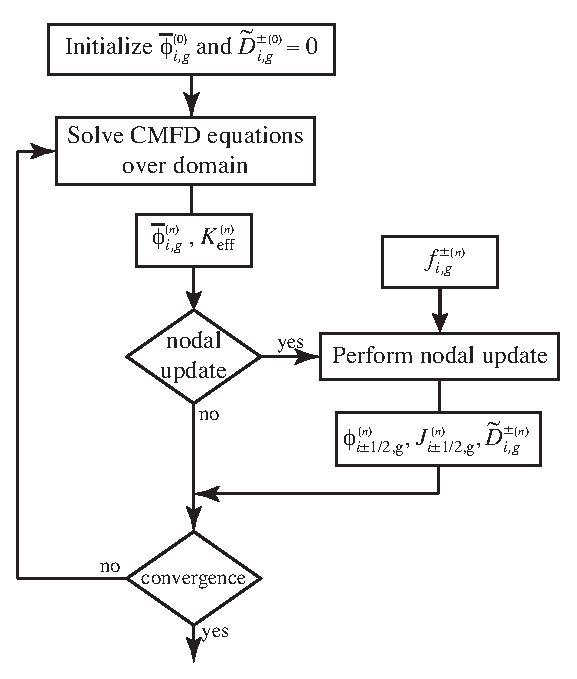
\includegraphics[scale=0.75]{./nodal_update.eps}
\parbox{11cm}{\caption{The nodal update procedure.}\label{fig:nodal_update}}   
\vspace{2pt}
\end{figure}
%

The analytic nodal method (ANM) is based on the {\sl Annals of Nuclear Energy} paper of Ref.~\citen{anm08}. The convergence of the ANM
relies on {\sl nodal correction iterations} consisting of repetitive solutions of the {\sl coarse mesh finite difference} (CMFD) method, as depicted in Fig.~\ref{fig:nodal_update}.
The CMFD method is similar to the {\sl mesh centered finite difference} (MCFD) method with the introduction of {\sl drift factors} $\tilde D_{i,g}^{\pm(n)}$ at each nodal correction
iteration. Solution of the CMFD equations relies on {\sl alternating direction implicit} (ADI) preconditionning with $LU$ factorization.

\goodbreak

The calling specifications are:

\begin{DataStructure}{Structure \dstr{NSSF:}}
\dusa{FLUX} \moc{:=} \moc{NSSF:} $[$ \dusa{FLUX} $]$ \dusa{TRACK} \dusa{MACRO} \moc{::} \dstr{NSSF\_data}
\end{DataStructure}

\noindent where
\begin{ListeDeDescription}{mmmmmm}

\item[\dusa{FLUX}] {\tt character*12} name of the {\sc lcm} object (type {\tt L\_FLUX}) containing the solution. If \dusa{FLUX} appears on the RHS, the solution previously stored in \dusa{FLUX}
is used to initialize the new iterative process; otherwise, a uniform unknown vector is used.

\item[\dusa{TRACK}] {\tt character*12} name of the {\sc lcm} object (type {\tt L\_TRACK}) containing the {\sc tracking}.

\item[\dusa{MACRO}] {\tt character*12} name of the {\sc lcm} object (type {\tt L\_MACROLIB}) containing the cross sections, diffusion coefficients and discontinuity
factors.

\item[\dstr{NSSF\_data}] structure containing the data to module {\tt NSSF:} (see Sect.~\ref{sect:nssf_data}).

\end{ListeDeDescription}

\vskip 0.2cm

\subsubsection{Data input for module {\tt NSSF:}}\label{sect:nssf_data}

\begin{DataStructure}{Structure \dstr{NSSF\_data}}
$[$ \moc{EDIT} \dusa{iprint} $]$ \\
$[~\{$ \moc{VAR1} $|$ \moc{ACCE} $\}$ \dusa{icl1} \dusa{icl2} $]$ \\
$[$ \moc{ADI} \dusa{nadi} $]$ \\
$[$ \moc{NUPD} $[$ \dusa{max\_no\_nodal\_iter} $[$ \dusa{no\_transverse\_iter} $]~]~[$ \dusa{nodal\_tol} $]~]$ \\
$[$ \moc{EXTE} $[$ \dusa{max\_no\_outer\_iter} $]~[$ \dusa{outer\_tol} $]~]$ \\
$[$ \moc{THER} $[$ \dusa{max\_no\_group\_iter} $]~[$ \dusa{group\_tol} $]~]$ \\
$[$ \moc{NODF} $]$ \\
$[$ \moc{LEAK} $\{$ \moc{flat} $|$ \moc{quadratic} $\}~]$ \\
$[$ \moc{BUCK} \dusa{valb2} $]$  \\
;
\end{DataStructure}

\noindent where
\begin{ListeDeDescription}{mmmmmm}

\item[\moc{EDIT}] keyword used to set \dusa{iprint}.

\item[\dusa{iprint}] index used to control the printing  in module {\tt NSSF:}.
=0 for no print; =1 for minimum printing (default value).

\item[\moc{VAR1}] keyword used to set the parameters \dusa{icl1} and \dusa{icl2}. These parameter are used with the symmetrical variational
acceleration technique (SVAT) for convergence of the generalized CMFD eigenvalue problem (default option) and to accelerate up-scattering iterations.

\item[\moc{ACCE}] alias keyword for \moc{VAR1}.

\item[\dusa{icl1}] number of free outer iterations in a cycle of the variational acceleration technique.
The default value is \dusa{icl1} $=3$.

\item[\dusa{icl2}] number of accelerated outer iterations  in a cycle of the
variational acceleration technique. The default value is \dusa{icl2} $=3$. A convergence in free iterations is
obtained by setting \dusa{icl1} $=200$ (or \dusa{icl1} $=$ \dusa{max\_no\_outer\_iter}) and \dusa{icl2} $=0$.

\item[\moc{ADI}] keyword to set the number of ADI iterations at the inner CMFD iterative level.

\item[\dusa{nadi}] number of ADI iterations (default: \dusa{nadi} $=2$).

\item[\moc{NUPD}] keyword to specify the maximum number of nodal update iterations. 

\item[\dusa{max\_no\_nodal\_iter}] maximum number of nodal update iterations iterations. The fixed default
value is \dusa{max\_no\_outer\_iter} $=300$.

\item[\dusa{no\_transverse\_iter}] number of tranverse current iterations in each nodal update iteration. We recommend to use the minimum value required for convergence of nodal update iterations. The fixed default
value is \dusa{no\_transverse\_iter} $=3$.

\item[\dusa{nodal\_tol}] convergence criterion for the nodal update iterations. The
fixed default value is \dusa{nodal\_tol} $=1.0\times 10^{-6}$.

\item[\moc{EXTE}] keyword to specify that the control parameters for the $K_{\rm eff}$ CMFD iteration are to be modified. 

\item[\dusa{max\_no\_outer\_iter}] maximum number of $K_{\rm eff}$ iterations. The fixed default
value is \dusa{max\_no\_outer\_iter} $=100$.

\item[\dusa{outer\_tol}] convergence criterion for the $K_{\rm eff}$ iterations. The
fixed default value is \dusa{outer\_tol} $=1.0\times 10^{-5}$.

\item[\moc{THER}] keyword to specify that the control parameters for the
thermal upscattering iteration are to be modified. 

\item[\dusa{max\_no\_group\_iter}] maximum number of thermal upscattering iterations. The fixed default
value is \dusa{max\_no\_group\_iter} $=0$.

\item[\dusa{group\_tol}] convergence criterion for the thermal upscattering iterations. The
fixed default value is \dusa{group\_tol} $=1.0\times 10^{-6}$.

\item[\moc{NODF}] keyword used to force discontinuity factors to one.

\item[\moc{LEAK}] keyword to specify the type of transverse leakage approximation.

\item[\moc{flat}] flat leakage approximation.

\item[\moc{quadratic}] quadratic leakage approximation in the internal nodes and linear leakage approximation in the boundary nodes.

\item[\moc{BUCK}] keyword used to specify the fixed buckling. By default,
\dusa{valb2} $=0$ cm$^{-2}$

\item[\dusa{valb2}] value of the fixed total buckling in cm$^{-2}$.

\end{ListeDeDescription}

\clearpage

\section{EXAMPLES OF INPUT DATA FILES}

\subsection{IAEA-2D benchmark}

The IAEA-2D benchmark is defined in Refs.~\citen{bivac,anl} and its geometry is represented in Fig.~\fig(iaea2d). Here, it is solved using a parabolic variational collocation method without mesh splitting of the elements:

\begin{figure}[htbp]
\begin{center} 
\epsfxsize=8.0cm
\centerline{ \epsffile{iaea2d.eps}}
\parbox{14cm}{\caption{Description of the IAEA-2D benchmark.}\label{fig:iaea2d}}  \end{center} 
\end{figure}

\begin{verbatim}
LINKED_LIST IAEA MACRO TRACK SYSTEM FLUX EDIT ;
MODULE GEO: MAC: TRIVAT: TRIVAA: FLUD: OUT: END: ;
*
IAEA := GEO: :: CAR2D 9 9
           EDIT 2
           X- DIAG X+ VOID
           Y- SYME Y+ DIAG
           MIX  3 2 2 2 3 2 2 1 4
                  2 2 2 2 2 2 1 4
                    2 2 2 2 1 1 4
                      2 2 2 1 4 4
                        3 1 1 4 0
                          1 4 4 0
                            4 0 0
                              0 0
                                0
           MESHX 0.0 20.0 40.0 60.0 80.0 100.0 120.0 140.0 160.0 180.0
           ;
MACRO := MAC: ::
 EDIT 2 NGRO 2 NMIX 4
 READ INPUT
 MIX     1
      DIFF  1.500E+00  4.0000E-01
     TOTAL  3.012E-02  8.0032E-02
    NUSIGF  0.000E+00  1.3500E-01
  H-FACTOR  0.000E+00  1.3500E-01
      SCAT  1 1 0.0 2 2 0.0 0.2E-01
 MIX     2
      DIFF  1.500E+00  4.0000E-01
     TOTAL  3.012E-02  8.5032E-02
    NUSIGF  0.000E+00  1.3500E-01
  H-FACTOR  0.000E+00  1.3500E-01
      SCAT  1 1 0.0 2 2 0.0 0.2E-01
 MIX     3
      DIFF  1.500E+00  4.00000E-01
     TOTAL  3.012E-02  1.30032E-01
    NUSIGF  0.000E+00  1.35000E-01
  H-FACTOR  0.000E+00  1.35000E-01
      SCAT  1 1 0.0 2 2 0.0 0.2E-01
 MIX     4
      DIFF  2.000E+00  3.0000E-01
     TOTAL  4.016E-02  1.0024E-02
      SCAT  1 1 0.0 2 2 0.0 0.4E-01
 ;
TRACK := TRIVAT: IAEA ::
      TITLE 'IAEA-2D BENCHMARK'
      MAXR 81 PRIM 2 ;
SYSTEM := TRIVAA: MACRO TRACK :: ;
FLUX := FLUD: SYSTEM ::
      EDIT 2 ;
EDIT := OUT: FLUX ::
       EDIT 2 INTG
       1  2  3  4  5  6  7  8  0
          9 10 11 12 13 14 15  0
            16 17 18 19 20 21  0
               22 23 24 25  0  0
                  26 27 28  0  0
                     29  0  0  0
                         0  0  0
                            0  0
                               0
       ;
END: ;
\end{verbatim}

\subsection{Biblis-2D benchmark}

The rods-withdrawn configuration of the Biblis-2D benchmark is defined in Ref.~\citen{bivac} and its geometry is represented in Fig.~\fig(biblis). Here, it is solved using a parabolic variational collocation method without mesh splitting of the elements:

\begin{figure}[htbp]
\begin{center} 
\epsfxsize=8.0cm
\centerline{ \epsffile{biblis.eps}}
\parbox{14cm}{\caption{Description of the Biblis-2D benchmark, rods-withdrawn configuration.}\label{fig:biblis}}  \end{center} 
\end{figure}

\begin{verbatim}
LINKED_LIST BIBLIS MACRO TRACK SYSTEM FLUX EDIT ;
MODULE GEO: MAC: TRIVAT: TRIVAA: FLUD: OUT: END: ;
*
BIBLIS := GEO: :: CAR2D 9 9
           EDIT 2
           X- DIAG X+ VOID
           Y- SYME Y+ DIAG
       MIX 1 8 2 6 1 7 1 4 3
             1 8 2 8 1 1 4 3
               1 8 2 7 1 4 3
                 2 8 1 8 4 3
                   2 5 4 3 3
                     4 4 3 0
                       3 3 0
                         0 0
                           0
       MESHX 0.0 23.1226 46.2452 69.3678 92.4904 115.613 138.7356
             161.8582 184.9808 208.1034
       ;
MACRO := MAC: ::
 EDIT 2 NGRO 2 NMIX 8
 READ INPUT
 MIX     1
      DIFF  1.436000E+00  3.635000E-01
     TOTAL  2.725820E-02  7.505800E-02
    NUSIGF  5.870800E-03  9.606700E-02
  H-FACTOR  2.376800E-03  3.889400E-02
      SCAT  1 1 0.0 2 2 0.0  1.775400E-02
 MIX     2
      DIFF  1.436600E+00  3.636000E-01
     TOTAL  2.729950E-02  7.843600E-02
    NUSIGF  6.190800E-03  1.035800E-01
  H-FACTOR  2.506400E-03  4.193500E-02
      SCAT  1 1 0.0 2 2 0.0  1.762100E-02
 MIX     3
      DIFF  1.320000E+00  2.772000E-01
     TOTAL  2.576220E-02  7.159600E-02
      SCAT  1 1 0.0 2 2 0.0  2.310600E-02
 MIX     4
      DIFF  1.438900E+00  3.638000E-01
     TOTAL  2.746400E-02  9.140800E-02
    NUSIGF  7.452700E-03  1.323600E-01
  H-FACTOR  3.017300E-03  5.358700E-02
      SCAT  1 1 0.0 2 2 0.0  1.710100E-02
 MIX     5
      DIFF  1.438100E+00  3.665000E-01
     TOTAL  2.729300E-02  8.482800E-02
    NUSIGF  6.190800E-03  1.035800E-01
  H-FACTOR  2.506400E-03  4.193500E-02
      SCAT  1 1 0.0 2 2 0.0  1.729000E-02
 MIX     6
      DIFF  1.438500E+00  3.665000E-01
     TOTAL  2.732400E-02  8.731400E-02
    NUSIGF  6.428500E-03  1.091100E-01
  H-FACTOR  2.602600E-03  4.417400E-02
      SCAT  1 1 0.0 2 2 0.0  1.719200E-02
 MIX     7
      DIFF  1.438900E+00  3.679000E-01
     TOTAL  2.729000E-02  8.802400E-02
    NUSIGF  6.190800E-03  1.035800E-01
  H-FACTOR  2.506400E-03  4.193500E-02
      SCAT  1 1 0.0 2 2 0.0  1.712500E-02
 MIX     8
      DIFF  1.439300E+00  3.680000E-01
     TOTAL  2.732100E-02  9.051000E-02
    NUSIGF  6.428500E-03  1.091100E-01
  H-FACTOR  2.602600E-03  4.417400E-02
      SCAT  1 1 0.0 2 2 0.0  1.702700E-02
       ;
TRACK := TRIVAT: BIBLIS ::
      TITLE 'BIBLIS BENCHMARK'
      EDIT 5 MAXR 81 PRIM 2 ;
SYSTEM := TRIVAA: MACRO TRACK ::
      EDIT 5 ;
FLUX := FLUD: SYSTEM ::
      EDIT 2 ;
EDIT := OUT: FLUX ::
       EDIT 2 INTG
       1  2  3  4  5  6  7  8  0
          9 10 11 12 13 14 15  0
            16 17 18 19 20 21  0
               22 23 24 25 26  0
                  27 28 29  0  0
                     30 31  0  0
                         0  0  0
                            0  0
                               0
       ;
END: ;
\end{verbatim}
\eject

\subsection{IAEA-3D benchmark}

The IAEA-3D benchmark is defined in Ref.~\citen{anl} and its geometry is represented in Fig.~\fig(iaea3d). Here, it is solved using a cubic mixed-dual method with mesh splitting of the second axial plane:

\begin{figure}[htbp]
\begin{center} 
\epsfxsize=15cm
\centerline{ \epsffile{iaea3d.eps}}
\parbox{14cm}{\caption{Description of the IAEA-3D benchmark.}\label{fig:iaea3d}}  \end{center} 
\end{figure}

\begin{verbatim}
LINKED_LIST IAEA3D MACRO TRACK SYSTEM FLUX EDIT ;
MODULE GEO: MAC: TRIVAT: TRIVAA: FLUD: OUT: END: ;
*
IAEA3D := GEO: :: CAR3D 9 9 4
          EDIT 2
          X- DIAG  X+ VOID 
          Y- SYME  Y+ DIAG 
          Z- VOID  Z+ VOID 
          MESHX 0.0 20.0 40.0 60.0 80.0 100.0 120.0 140.0 160.0 180.0 
          MESHZ 0.0 20.0 280.0 360.0 380.0 
          SPLITZ 1 2 1 1
          (* PLANE NB 1 *) 
          MIX 4 4 4 4 4 4 4 4 4 
                4 4 4 4 4 4 4 4 
                  4 4 4 4 4 4 4 
                    4 4 4 4 4 4 
                      4 4 4 4 0 
                        4 4 4 0 
                          4 0 0 
                            0 0 
                              0 
              (* PLANE NB 2 *) 
              3 2 2 2 3 2 2 1 4 
                2 2 2 2 2 2 1 4 
                  2 2 2 2 1 1 4 
                    2 2 2 1 4 4 
                      3 1 1 4 0 
                        1 4 4 0 
                          4 0 0 
                            0 0 
                              0 
              (* PLANE NB 3 *) 
              3 2 2 2 3 2 2 1 4 
                2 2 2 2 2 2 1 4 
                  3 2 2 2 1 1 4 
                    2 2 2 1 4 4 
                      3 1 1 4 0 
                        1 4 4 0 
                          4 0 0 
                            0 0 
                              0 
              (* PLANE NB 4 *) 
              5 4 4 4 5 4 4 4 4 
                4 4 4 4 4 4 4 4 
                  5 4 4 4 4 4 4 
                    4 4 4 4 4 4 
                      5 4 4 4 0 
                        4 4 4 0 
                          4 0 0 
                            0 0 
                              0 
           ;
MACRO := MAC: ::
 EDIT 2 NGRO 2 NMIX 5
 READ INPUT
 MIX     1
      DIFF  1.500E+00  4.0000E-01
     TOTAL  3.000E-02  8.0000E-02
    NUSIGF  0.000E+00  1.3500E-01
  H-FACTOR  0.000E+00  1.3500E-01
      SCAT  1 1 0.0 2 2 0.0 0.2E-01
 MIX     2
      DIFF  1.500E+00  4.0000E-01
     TOTAL  3.000E-02  8.5000E-02
    NUSIGF  0.000E+00  1.3500E-01
  H-FACTOR  0.000E+00  1.3500E-01
      SCAT  1 1 0.0 2 2 0.0 0.2E-01
 MIX     3
      DIFF  1.500E+00  4.00000E-01
     TOTAL  3.000E-02  1.30000E-01
    NUSIGF  0.000E+00  1.35000E-01
  H-FACTOR  0.000E+00  1.35000E-01
      SCAT  1 1 0.0 2 2 0.0 0.2E-01
 MIX     4
      DIFF  2.000E+00  3.0000E-01
     TOTAL  4.000E-02  1.0000E-02
      SCAT  1 1 0.0 2 2 0.0 0.4E-01
 MIX     5
      DIFF  2.000E+00  3.0000E-01
     TOTAL  4.000E-02  5.5000E-02
      SCAT  1 1 0.0 2 2 0.0 0.4E-01
 ;
TRACK := TRIVAT: IAEA3D ::
      TITLE 'TEST IAEA 3D'
      EDIT 5 MAXR 405 DUAL 3 1 ;
SYSTEM := TRIVAA: MACRO TRACK ::
      EDIT 5 ;
FLUX := FLUD: SYSTEM ::
      EDIT 2 ;
EDIT := OUT: FLUX ::
       EDIT 2 INTG
       (* PLANE NB 1 *) 
       0  0  0  0  0  0  0  0  0 
          0  0  0  0  0  0  0  0 
             0  0  0  0  0  0  0 
                0  0  0  0  0  0 
                   0  0  0  0  0
                      0  0  0  0
                         0  0  0
                            0  0
                               0
       (* PLANE NB 2 *) 
       1  2  3  4  5  6  7  8  0 
          9 10 11 12 13 14 15  0 
            16 17 18 19 20 21  0 
               22 23 24 25  0  0 
                  26 27 28  0  0
                     29  0  0  0
                         0  0  0
                            0  0
                               0
       (* PLANE NB 3 *) 
       30 31 32 33 34 35 36 37  0 
          38 39 40 41 42 43 44  0 
             45 46 47 48 49 50  0 
                51 52 53 54  0  0 
                   55 56 57  0  0
                      58  0  0  0
                          0  0  0
                             0  0
                                0
       (* PLANE NB 4 *) 
       0  0  0  0  0  0  0  0  0 
          0  0  0  0  0  0  0  0 
             0  0  0  0  0  0  0 
                0  0  0  0  0  0 
                   0  0  0  0  0
                      0  0  0  0
                         0  0  0
                            0  0
                               0
       ;
END: ;
\end{verbatim}

\subsection{S30 hexagonal benchmark in 2-D}

The S30 hexagonal benchmark in 2-D is defined in Ref.~\citen{benaboud}. Its geometry is represented in Fig.~\fig(hexS30). Here, it is solved using a mesh centered finite difference method without mesh splitting of the hexagonal elements:

\begin{figure}[htbp]
\begin{center} 
\epsfxsize=6cm
\centerline{ \epsffile{hexS30.eps}}
\parbox{14cm}{\caption{Description of the S30 hexagonal benchmark.}\label{fig:hexS30}}  \end{center} 
\end{figure}

\begin{verbatim}
LINKED_LIST HEX MACRO TRACK SYSTEM FLUX EDIT ;
MODULE GEO: MAC: TRIVAT: TRIVAA: FLUD: OUT: END: ;
*
HEX := GEO: :: HEX   6
       EDIT 2
       HBC S30 ZERO
       SIDE 13.044
       SPLITH 0
       MIX
       1
       2
       2  2
       3  3
       ;
MACRO := MAC: ::
 EDIT 2 NGRO 2 NMIX 3
 READ INPUT
 MIX     1
      DIFF  1.5E+00  4.00E-01
     TOTAL  3.0E-02  1.30E-01
    NUSIGF  0.0E+00  1.35E-01
  H-FACTOR  0.0E+00  1.35E-01
      SCAT  1 1 0.0 2 2 0.0  0.2E-01
 MIX     2
      DIFF  1.5E+00  4.00E-01
     TOTAL  3.0E-02  8.50E-02
    NUSIGF  0.0E+00  1.35E-01
  H-FACTOR  0.0E+00  1.35E-01
      SCAT  1 1 0.0 2 2 0.0  0.2E-01
 MIX     3
      DIFF  2.0E+00  3.0E-01
     TOTAL  4.0E-02  1.0E-02
      SCAT  1 1 0.0 2 2 0.0  0.4E-01
 ;
TRACK := TRIVAT: HEX ::
      TITLE 'S30 HEXAGONAL BENCHMARK IN 2-D.'
      EDIT 5 MAXR 50 MCFD (* IELEM= *) 1 ;
SYSTEM := TRIVAA: MACRO TRACK ::
      EDIT 5 ;
FLUX := FLUD: SYSTEM ::
      EDIT 2 ;
EDIT := OUT: FLUX ::
       EDIT 2 INTG IN ;
END: ;
\end{verbatim}

\subsection{LMW benchmark in 2-D}

The LMW benchmark in 2-D is a space-time kinetics problem introduced by Greenman\cite{greenman} and used by Monier\cite{monier}.
Its geometry is represented in Fig.~\fig(lmw). Here, it is solved using a parabolic nodal collocation method with $2\times 2$ mesh splitting
of each element. A reactivity transient is induced by the rapid withdrawal of the control rod in material mixture 6. The control rod is
removed in 26.7 s, causing a negative ramp variation in total cross section.

\begin{figure}[htbp]
\begin{center} 
\epsfxsize=7cm
\centerline{ \epsffile{lmw.eps}}
\parbox{14cm}{\caption{Description of the LMW benchmark in 2-D.}\label{fig:lmw}}  \end{center} 
\end{figure}

\goodbreak
\begin{verbatim}
*----
*  TEST CASE LMW 2D
*
*  REF: G. Greenman, "A Quasi-Static Flux Synthesis Temporal Integration
*       Scheme for an Analytic Nodal Method," Nuclear Engineer's Thesis,
*       Massachusetts Institute of Technology, Department of Nuclear
*       Engineering (May 1980).
*
*----
*  Define STRUCTURES and MODULES used
*----
LINKED_LIST LMW TRACK MACRO1 SYSTEM1 MACRO2 SYSTEM2 FLUX KINET ;
MODULE GEO: MAC: TRIVAT: TRIVAA: FLUD: INIKIN: KINSOL: GREP: DELETE:
       END: ;
REAL fnorm sigt1 sigt2 ;
REAL TIME := 0.0 ;
PROCEDURE assertS assertS2 ;
*
LMW := GEO: :: CAR2D 6 6
      X- REFL X+ ZERO
      Y- REFL Y+ ZERO
      MIX 1 1 1 2 3 4
          1 1 1 1 3 4
          1 1 5 1 3 4
          6 1 1 3 3 4
          3 3 3 3 4 4
          4 4 4 4 4 0
      MESHX  0.0 10. 30. 50. 70. 90. 110.
      MESHY  0.0 10. 30. 50. 70. 90. 110.
      SPLITX 2 2 2 2 2 2
      SPLITY 2 2 2 2 2 2
      ;
MACRO1 := MAC: ::
 EDIT 0 NGRO 2 NMIX 6
 READ INPUT
 MIX     1
      DIFF  1.423910E+00  3.563060E-01
     TOTAL  2.795756E-02  8.766216E-02
    NUSIGF  6.477691E-03  1.127328E-01
  H-FACTOR  2.591070E-03  4.509310E-02
      SCAT  1 1 0.0 2 2 0.0  0.175555E-01
      OVERV 0.800E-07  4.000E-06
 MIX     2
      DIFF  1.423910E+00  3.563060E-01
     TOTAL  2.850756E-02  9.146219E-02
    NUSIGF  6.477691E-03  1.127328E-01
  H-FACTOR  2.591070E-03  4.509310E-02
      SCAT  1 1 0.0 2 2 0.0  0.175555E-01
      OVERV 0.800E-07  4.000E-06
 MIX     3
      DIFF  1.425610E+00  3.505740E-01
     TOTAL  2.817031E-02  9.925634E-02
    NUSIGF  7.503282E-03  1.378004E-01
  H-FACTOR  3.001310E-03  5.512106E-02
      SCAT  1 1 0.0 2 2 0.0  0.171777E-01
      OVERV 0.800E-07  4.000E-06
 MIX     4
      DIFF  1.634220E+00  2.640020E-01
     TOTAL  3.025750E-02  4.936351E-02
      SCAT  1 1 0.0 2 2 0.0  0.275969E-01
      OVERV 0.800E-07  4.000E-06
 MIX     5
      DIFF  1.423910E+00  3.563060E-01
     TOTAL  2.795756E-02  8.766216E-02
    NUSIGF  6.477691E-03  1.127328E-01
  H-FACTOR  2.591070E-03  4.509310E-02
      SCAT  1 1 0.0 2 2 0.0  0.175555E-01
      OVERV 0.800E-07  4.000E-06
 MIX     6
      DIFF  1.423910E+00  3.563060E-01
     TOTAL  2.850756E-02  9.146217E-02
    NUSIGF  6.477691E-03  1.127328E-01
  H-FACTOR  2.591070E-03  4.509310E-02
      SCAT  1 1 0.0 2 2 0.0  0.175555E-01
      OVERV 0.800E-07  4.000E-06
 ;
TRACK := TRIVAT: LMW ::
      TITLE 'LMW 2-D BENCHMARK'
      EDIT 1 MAXR 144 MCFD 2 ;
SYSTEM1 := TRIVAA: MACRO1 TRACK ::
      EDIT 1 UNIT ;
FLUX := FLUD: SYSTEM1 TRACK ::
      EDIT 1 EXTE 5.0E-7 ;
assertS FLUX :: 'K-EFFECTIVE' 1 1.014803 ;
*----
*  Crank-Nicholson space-time kinetics
*----
EVALUATE TIME := 0.0 ;
KINET := INIKIN: MACRO1 TRACK SYSTEM1 FLUX :: EDIT 1
      NDEL 6
      BETA   0.000247 0.0013845 0.001222 0.0026455 0.000832 0.000169
      LAMBDA 0.0127 0.0317 0.115 0.311 1.40 3.87    
      CHID   1.0 1.0 1.0 1.0 1.0 1.0
             0.0 0.0 0.0 0.0 0.0 0.0
      NORM POWER-INI 1.0E4 ;
EVALUATE sigt1 := 2.850756E-02 ;
EVALUATE sigt2 := 9.146217E-02  ;
WHILE TIME 26.7 <= DO
  EVALUATE sigt1 := sigt1 5.5E-4 0.1 26.7 / * - ;
  EVALUATE sigt2 := sigt2 3.8E-3 0.1 26.7 / * - ;
  MACRO2 := MAC: MACRO1 ::
      EDIT 0
      READ INPUT
      MIX     6
         TOTAL  <<sigt1>>  <<sigt2>>
      ;
  SYSTEM2 := TRIVAA: MACRO2 TRACK ::
      EDIT 1 UNIT ;
  KINET := KINSOL: KINET MACRO2 TRACK SYSTEM2 MACRO1 SYSTEM1 ::
      EDIT 5  DELTA 0.1 
      SCHEME  FLUX CRANK PREC CRANK EXTE 1.0E-6 ;
  GREP: KINET :: GETVAL 'TOTAL-TIME' 1 >>TIME<< ;
  ECHO "TIME=" TIME "S" "sigt=" sigt1 sigt2 ;
  IF TIME 1.0 - ABS 1.0E-3 < THEN
    assertS2 KINET :: 'CTRL-FLUX' 1 1.986270E+02 ;
    assertS2 KINET :: 'CTRL-PREC' 1 1.095509E-01 ;
    assertS2 KINET :: 'E-POW'     1 1.008753E+04 ;
  ELSEIF TIME 5.0 - ABS 1.0E-3 < THEN
    assertS2 KINET :: 'CTRL-FLUX' 1 2.090369E+02 ;
    assertS2 KINET :: 'CTRL-PREC' 1 1.097266E-01 ;
    assertS2 KINET :: 'E-POW'     1 1.063990E+04 ;
  ELSEIF TIME 10.0 - ABS 1.0E-3 < THEN
    assertS2 KINET :: 'CTRL-FLUX' 1 2.305455E+02 ;
    assertS2 KINET :: 'CTRL-PREC' 1 1.104699E-01 ;
    assertS2 KINET :: 'E-POW'     1 1.176902E+04 ;
  ELSEIF TIME 15.0 - ABS 1.0E-3 < THEN
    assertS2 KINET :: 'CTRL-FLUX' 1 2.641221E+02 ;
    assertS2 KINET :: 'CTRL-PREC' 1 1.121002E-01 ;
    assertS2 KINET :: 'E-POW'     1 1.352433E+04 ;
  ELSEIF TIME 20.0 - ABS 1.0E-3 < THEN
    assertS2 KINET :: 'CTRL-FLUX' 1 3.157370E+02 ;
    assertS2 KINET :: 'CTRL-PREC' 1 1.150681E-01 ;
    assertS2 KINET :: 'E-POW'     1 1.621938E+04 ;
  ELSEIF TIME 25.0 - ABS 1.0E-3 < THEN
    assertS2 KINET :: 'CTRL-FLUX' 1 3.971426E+02 ;
    assertS2 KINET :: 'CTRL-PREC' 1 1.200883E-01 ;
    assertS2 KINET :: 'E-POW'     1 2.047011E+04 ;
  ELSEIF TIME 26.7 - ABS 1.0E-3 < THEN
    assertS2 KINET :: 'CTRL-FLUX' 1 4.351272E+02 ;
    assertS2 KINET :: 'CTRL-PREC' 1 1.224600E-01 ;
    assertS2 KINET :: 'E-POW'     1 2.245449E+04 ;
  ENDIF ;
  MACRO1 SYSTEM1 := DELETE: MACRO1 SYSTEM1 ;
  MACRO1 := MACRO2 ;
  SYSTEM1 := SYSTEM2 ;
  MACRO2 SYSTEM2 := DELETE: MACRO2 SYSTEM2 ;
ENDWHILE ;
ECHO "test lmw2D completed" ;
\end{verbatim}

\clearpage
\phantomsection
\begin{thebibliography}{99}

\bibitem{PIP2009}
A. H\'EBERT, {\sl Applied Reactor Physics}, Second Edition, Presses Internationales Polytechnique, ISBN 978-2-553-01698-1, 396 p., Montr\'eal, 2016.

\bibitem{cle2000}
R.~ROY, \textsl{The CLE-2000 Tool-Box}, 
Report IGE--163, Institut de g\'enie nucl\'eaire, \'{E}cole Polytechnique de Montr\'eal,
Montr\'{e}al, Qu\'{e}bec (1999).

\bibitem{ganlib5}
A. H\'EBERT and R.~ROY,
``The Ganlib5 kernel guide (64--bit clean version),"
Report IGE-332, \'Ecole Polytechnique de Montr\'eal, January 2013.

\bibitem{bivac}
A. H\'EBERT, ``Application of the Hermite Method for Finite Element Reactor Calculations," {\sl Nucl. Sci. Eng.}, {\bf 91}, 34 (1985).

\bibitem{SVAT1}
A. H\'EBERT, ``Variational Principles and Convergence Acceleration Strategies for the Neutron Diffusion Equation,'' {\sl Nucl. Sci. Eng.}, {\bf 91}, 414 (1985).

\bibitem{SVAT2}
A. H\'EBERT, ``Preconditioning the Power Method for Reactor Calculations,'' {\sl Nucl. Sci. Eng.}, {\bf 94}, 1 (1986).

\bibitem{MCFD}
A. H\'EBERT, ``Development of the Nodal Collocation Method for Solving the Neutron Diffusion Equation,'' {\sl Ann. Nucl. Energy}, {\bf 14}, 527 (1987).

\bibitem{Trivac}
A. H\'EBERT, ``TRIVAC, A Modular Diffusion Code for Fuel Management and Design Applications,'' {\sl Nucl. J. of Canada}, Vol. 1, No. 4, 325 (1987).

\bibitem{mixte-dual}
A. H\'EBERT, ``Application of a Dual Variational Formulation to Finite Element Reactor Calculations,'' {\sl Ann. nucl. Energy}, {\bf 20}, 823 (1993).

\bibitem{nse2005}
A. H\'EBERT, ``The Search for Superconvergence in Spherical Harmonics Approximations,'' {\sl Nucl. Sci. Eng.}, {\bf 154}, 134 (2006).

\bibitem{ane10a}
A. H\'EBERT, ``Mixed-dual implementations of the of the simplified $P_n$ method," {\sl Ann. nucl. Energy}, {\bf 37}, 498 (2010).

\bibitem{iram}
J. BAGLAMA, ``Augmented Block Householder Arnoldi Method,"
{\sl Linear Algebra Appl.}, {\bf 429}, Issue 10, 2315--2334 (2008).

\bibitem{wilkinson}
J. H. WILKINSON, ``The Algebraic Eigenvalue Problem,'' {\sl Clarendon Press}, Oxford (1965).

\bibitem{roy}
R. ROY, Private communication.

\bibitem{monier}
A. MONIER, ``Application of the Collocation Technique to the Spatial Discretization of the Generalized Quasistatic Method for Nuclear Reactors," Ph. D. Thesis, Polytechnique Montr\'eal, Institut de G\'enie \'Energ\'etique (December 1991).

\bibitem{benaboud}
A. BENABOUD, ``R\'esolution de l'\'equation de la diffusion neutronique pour une g\'eom\'etrie hexagonale," Ph. D. Thesis, Polytechnique Montr\'eal, Institut de G\'enie \'Energ\'etique (December 1992).

\bibitem{rts}
A. H\'EBERT, ``A Raviart--Thomas--Schneider solution of the diffusion equation in hexagonal geometry", {\sl Ann. nucl. Energy},
{\bf 35}, 363 (2008).

\bibitem{recipes}
W. H. PRESS, S. A. TEUKOLSKY, W. T. VETTERLING and B. P. FLANNERY, ``Numerical Recipes in FORTRAN," Second Edition, Chapter 16, Cambridge University Press (1992).

\bibitem{cronos}
J. J. LAUTARD, S. LOUBI\`ERE and C. FEDON-MAGNAUD, ``CRONOS, a Computational Modular System for Neutronic Core Calculations," Proc. International Atomic Energy Agency Specialists Mtg. on Advanced Calculational Methods for Power Reactors, Cadarache, France, September 1990.

\bibitem{nestle}
P. J. TURINSKY, R. M. K. AL-CHALABI, P. ENGRAND, H. N. SARSOUR, F. X. FAURE and  W. GUO, ``NESTLE: Few-group neutron diffusion equation solver utilzing the nodal expansion
method for eigenvalue, adjoint, fixed-source steady-state and transient problem,'' Electric Power Research Center, North Carolina State University, Raleigh, NC 27695-7909 (1994).

\bibitem{anm08}
A. H\'EBERT, ``A simplified presentation of the multigroup analytic nodal method
in 2--D Cartesian geometry," {\sl Ann. nucl. Energy}, {\bf 35}, 2142--2149 (2008).

\bibitem{anl}
``Argonne Code Center: Benchmark Problem Book," ANL-7416, Supp. 2, ID11-A2, Argonne National Laboratory (1977).

\bibitem{greenman}
G. GREENMAN, ``A Quasi-Static Flux Synthesis Temporal Integration Scheme for an Analytic Nodal Method," Nuclear Engineer's Thesis, Massachusetts Institute of Technology, Department of Nuclear Engineering (May 1980).

\end{thebibliography}

\clearpage
\phantomsection
\printindex

\end{document}
